\documentclass[12pt,a4paper,TimesNewRoman]{article}
\usepackage{graphicx}
\usepackage[14pt]{extsizes}
\usepackage{cmap}
\usepackage[T2A]{fontenc}
\usepackage[utf8]{inputenc}
\usepackage[english,russian]{babel}
\usepackage[left=2.5cm,right=1.5cm,top=2cm,bottom=2cm]{geometry}
\linespread{1.3} %междустрочный интервал 1.5
%абзацный отступ 1.25??
%выравнивание по ширине??
\usepackage{indentfirst}
\usepackage{graphicx}
\usepackage{subcaption}
\usepackage{mathtools}
\usepackage{amsmath}
\usepackage{amssymb}
\usepackage{amsfonts}
\usepackage{float}
%\usepackage{caption}
\usepackage[unicode,pdftex]{hyperref}
\usepackage{polynom}
\usepackage{multicol}
\setcounter{page}{2}
\usepackage{enumitem}
\usepackage{listings}
\usepackage{courier} % Подключает гарнитуру Courier

% Настройка параметров листинга под твои требования
\lstset{
    basicstyle=\fontfamily{pcr}\fontsize{12pt}{14.4pt}\selectfont, % Courier (pcr), 12 пт
    frame=single,          % Одинарная рамка вокруг кода
    aboveskip=0pt,         % Интервал до абзаца - 0 пт
    belowskip=0pt,         % Интервал после абзаца - 0 пт
    lineskip=0pt,          % Межстрочный интервал (одинарный)
    xleftmargin=0pt,       % Выравнивание строго по левому краю (без отступов)
    breaklines=true,       % Автоматический перенос длинных строк
    showstringspaces=false,% Не отображать пробелы как подчеркивания
    tabsize=4,             % Размер табуляции (настраивается по вкусу)
    numbers=none           % Отключение нумерации строк (по ГОСТ чаще всего не нужна)
}

\usepackage[unicode, pdftex]{hyperref}
\hypersetup{
    colorlinks=true,    % Включает цветные ссылки вместо рамок
    linkcolor=black,    % Цвет внутренних ссылок (например, на разделы)
    urlcolor=black,     % Цвет URL-ссылок
    citecolor=black,    % Цвет ссылок на литературу
    pdfborder={0 0 0},  % Убирает рамки вокруг ссылок
    pdfstartview=FitH,  % Опция для правильного отображения при открытии
    bookmarksnumbered=true, % Нумерованные закладки в PDF
    bookmarksopen=true      % Раскрывать закладки по умолчанию
}

\usepackage{caption}
\DeclareCaptionFormat{custom}{#1#2~--- #3} % Формат: "Рисунок 1 — Текст"
\captionsetup[figure]{
    format=custom,
    name=Рисунок,
    labelsep=space, % Убирает двоеточие
}

\title{Выпускная квалификационная работа}
\author{Каплан Владислав}
\date{March 2026}

\begin{document}

\newpage
\section*{Реферат}


\thispagestyle{empty}
\tableofcontents
\newpage

\section*{Введение}
Современное развитие систем контрольно-измерительной аппаратуры, радиолокации и биомедицинской электроники требует формирования прецизионных сигналов не только стандартной формы, но и специальных и произвольных форм. Традиционные аналоговые решения постепенно вытесняются цифровыми системами, так как последние обеспечивают высокую повторяемость характеристик, гибкость настройки и устойчивость \cite{Hao_2021}.

Разработка генератора сигналов специальной формы (ГССФ) на базе программируемых логических интегральных схем (ПЛИС) является актуальной задачей, так как позволяет совместить скорость обработки данных, сопоставимую с аппаратными решениями и программную гибкость, присущую микропроцессорным системам.

Для решения задачи генерации сигналов традиционно рассматриваются три основных подхода:
\begin{enumerate}
    \item Аналоговый синтез (на основе интегральных генераторов). Минусами этого способа являются низкая стабильность частоты и громоздкость схемы при необходимости реализации нескольких типов сигналов.
    \item Косвенный цифровой синтез (на базе PLL/ФАПЧ). Несмотря на высокую чистоту спектра, системы на базе PLL обладают низкой скоростью перестройки частоты и фазы. Главный недостаток в контексте данной работы -- невозможность формирования произвольных форм сигнала без изменения аппаратной конфигурации или сложной обвязки.
    \item Прямой цифровой синтез (DDS -- Direct Digital Synthesis). Этот способ обеспечивает практически мгновенную перестройку частоты и фазы без разрыва фазы сигнала, позволяет воспроизводить сигналы любой формы, описанные математически или заданные набором точек в памяти.
\end{enumerate}
В условиях задачи, требующей регулировки амплитуды, смещения, скважности и воспроизведения сигналов произвольной формы, метод DDS в сочетании с архитектурой ПЛИС является оптимальный вариантом, обеспечивающим необходимую детерминированность и гибкость.

Целью выпускной квалификационной работы является разработка и аппаратно-программная реализация устройства генерации сигналов специальной формы на ПЛИС.
Основные задачи работы:
\begin{enumerate}
    \item Анализ технических характеристик ГССФ и уточнение требований к его реализации на основе ПЛИС.
    \item Анализ системы формирования частот в базисе ПЛИС.
    \item Разработка поведенческого описания ГССФ на основе ПЛИС.
    \item Моделирование ГССФ инструментами САПР Vivado.
    \item Тестовые испытания ГССФ на основе отладочной платы с ПЛИС. Демонстрация воспроизведения сигналов специальной формы.
\end{enumerate}

\section{Анализ методов построения и принципов реализации ГССФ}

\subsection{Общие принципы цифрового синтеза}
В современной микроэлектронике доминирующим подходом к построению прецизионных источников сигналов является цифровой синтез \cite{shunli}. В отличие от аналоговых автогенераторов, где частота определяется параметрами $L$ и $C$ элементов, цифровые системы используют стабильную тактовую частоту $f_{clk}$ опорного кварцевого резонатора и математические алгоритмы формирования отсчетов.

Для формирования сигналов специальной формы в базисе ПЛИС наиболее эффективными являются методы, основанные на циклическом переборе значений фазы \cite{tierney}.

\subsection{Алгоритм CORDIC для вычисления гармонических функций}
При реализации функции генерации синусоидального сигнала на базе ПЛИС, помимо классического табличного метода, применяется алгоритм CORDIC (Coordinate Rotation Digital Computer). Данный алгоритм представляет собой итерационный метод вычисления элементарных математических функций, включая тригонометрические, используя исключительно операции сложения и побитового сдвига \cite{cordic}.

В основе метода CORDIC лежит принцип вращения вектора в координнатной плоскости. На каждой итерации вектор поворачивается на заранее определенный угол. Для достижения $N$-битной точности требуется $N$ итераций, что на уровне RTL реализуется в виде конечного автомата, либо в виде конвейерного блока.

Пусть задан начальный вектор с координатами $(x_0, y_0)$. Поворот этого вектора на заданный угол $\theta$ приводит к новому вектору $(x_1, y_1)$, координаты которого определяются матрицей поворота $M(\theta)$:

\begin{equation} \label{eq:cordic1}
    M(\theta) =
    \begin{pmatrix}
        \cos\theta & \mp \sin\theta \\
        \pm \sin\theta & \cos \theta
    \end{pmatrix}
\end{equation}

Поворот выполняется путем умножения матрицы поворота \eqref{eq:cordic1} на вектор-столбец:
\begin{equation} \label{eq:cordic2}
    \begin{bmatrix}
        x_1 \\
        y_1
    \end{bmatrix} =
    \begin{bmatrix}
        \cos\theta & \mp \sin\theta \\
        \pm \sin\theta & \cos \theta
    \end{bmatrix}
    \begin{bmatrix}
        x_0 \\
        y_0
    \end{bmatrix}
\end{equation}

Координаты нового вектора $(x_1, y_1)$ в результате операции \eqref{eq:cordic2} имеют вид:
\begin{equation}\label{eq:cordic3}
    x_1 = x\cos\theta \mp y\sin\theta, \quad
    y_1 = \pm x\sin\theta + y\cos\theta
\end{equation}

Для аппаратной реализации вычисление синусов и косинусов, также как и операция умножения являются ресурсоемкими. Основная идея CORDIC заключается в преобразовании уравнений \eqref{eq:cordic3}, чтобы исключить эти операции.

Вынесем $\cos\theta$ за скобки:
\begin{equation} \label{eq:cordic4}
    x_1 = \cos\theta \cdot \left[x_0-y_0\tan(\theta)\right] \quad
    y_1 = \cos\theta \cdot \left[y_0+x_0\tan(\theta)\right]
\end{equation}

Алгоритм предполагает разбиение искомого угла $\theta$ на последовательность фиксированных углов $\alpha_i$, таких что их сумма приближается к $\theta$. Ключевым моментом является выбор $\alpha_i$ таким образом, чтобы тангес этих углов представлял собой степень двойки \cite{cordic}:
\begin{equation} \label{eq:cordic5}
    \tan(\alpha_i) = 2^{-i}, \quad \text{где } i=0,1,2, \dots, N-1
\end{equation}

Для цифровой реализации это означает что умножение на $\tan(\alpha_i)$ может быть заменено на тривиальную операцию арифметического сдвига вправо на $i$ разрядов. Таким образом, ресурсоемкие умножители заменяются на сдвиговые регистры. С учетом \eqref{eq:cordic5}, уравнение $i$-й итерации принимает вид:
\begin{equation} \label{eq:cordic6}
    x_{i+1} = K_i \cdot \left[x_i - d_i \cdot y_i \cdot 2^{-i}\right], \quad
    y_{i+1} = K_i \cdot \left[y_i + d_i \cdot x_i \cdot 2^{-i}\right]
\end{equation}

Где $d_i \in {-1,1}$ - направление вращения на $i$-й итерации. Выбор направления зависит от разности между целевым углом $\theta$ и текущим накопленным углом $z_i$. Для отслеживания разности между ними используется третье уравнения - аккумулятор фазовой ошибки \cite{cordic}:

\begin{equation} \label{eq:cordic7}
    z_{i+1} = z_i - d_i \cdot \alpha_i = z_i - d_i \cdot \arctan(2^{-i})
\end{equation}

Направление вращения $d_i$ определяется знаком $z_i$:
\begin{equation}
    d_i =
    \begin{cases}
        1, & \text{если } z_i \ge 0 \\
        -1, & \text{если } z_i < 0
    \end{cases}
\end{equation}

Коэффициент $K_i$ в уравнениях \eqref{eq:cordic6} представляет собой коэффициент деформации, возникающий из-за отбрасывания умножения на $\cos\alpha_i$ на каждой итерации при вычислении сдвигов:
\begin{equation}
    K_i = cos(\alpha_i) = \frac{1}{\sqrt{1 + \tan^2(\alpha_i)}} = \frac{1}{\sqrt{1 + 2^{-2i}}}
\end{equation} 

Поскольку последовательность углов поворота фиксирована, общее изменения масштаба вектора за N итераций является константой, которую можно рассчитать заранее:
\begin{equation}
    K = \prod_{i=0}^{N-1} K_i = \prod_{i=0}^{N-1} \frac{1}{\sqrt{1 + 2^{-2i}}}
\end{equation}

\subsubsection{Режим вычисления синуса и косинуса}

Для генерации гармонических сигналов алгоритм CORDIC используется в режиме вращения \cite{cordic}. В качестве начальных условий задаются:
\begin{itemize}
    \item $x_0 = K^{-1}$ - начальное значение по оси $x$, компенсирующее коэффициент деформации;
    \item $y_0 = 0$;
    \item $z_0 = \theta$ - целевой угол, который соответствует текущему значению фазы из фазового аккумулятора.
\end{itemize}

После выполнения $N$ итераций, значение фазовой ошибки $z_N$ стремится к нулю, а координаты вектора содержат искомые значения:

\begin{equation}
    x_N \approx \cos\theta, \quad y_N \approx \sin\theta
\end{equation}

Таким образом, для аппаратной реализации генератора синусоидального сигнала требуется лишь логика управления знаком, сумматоры, блоки побитового сдвига и регистры для хранения промежуточных результатов, что делает алгоритм CORDIC эффективным решением для ПЛИС.

\subsection{Метод прямого цифрового синтеза}
Принцип DDS (Direct Digital Synthesis) основан на генерации последовательности цифровых отсчетов сигнала путем обращения к таблице соответствия "фаза-амплитуда".

Основным узлом DDS-генератора является фазовый аккумулятор разрядностью $M$. На каждом такте системной частоты $f_{clk}$ к текущему значению аккумулятора прибавляется код приращения фазы $\Delta \Theta$. Выходное значение аккумулятора представляет собой линейно растущую фазу $\phi(n)$.

\begin{figure}[H]
    \centering
    
\includegraphics[width=0.9\linewidth]{/home/buba/Documents/fpga-waveform-generator/text/assets/dds-functional.png}
    \caption{Функциональная блок-схема системы DDS \cite{analog-dds}}
    \label{fig:1}
\end{figure}

\begin{figure}[h]
    \centering
    
\includegraphics[width=0.9\linewidth]{/home/buba/Documents/fpga-waveform-generator/text/assets/typical-dds.png}
    \caption{Типичная архитектура DDS и путь передачи сигнала с ЦАП \cite{analog-dds}}
    \label{fig:2}
\end{figure}

Связь между выходной частотой $f_{out}$ и приращением фазы описывается уравнением \cite{shunli}:
\begin{equation} \label{eq:1}
    f_{out}=\frac{\Delta \Theta \cdot f_{clk}}{2^M}
\end{equation}

Разрешение по частоте определяется как:
\begin{equation} \label{eq:2}
    \delta f = \frac{f_{clk}}{2^M}
\end{equation}

Таким образом, при использовании 32-битного аккумулятора фазы ($M=32$) и частоты тактирования 100 МГц, разрешение по частоте составит:
\begin{equation}
    \delta f = \frac{100\cdot10^6}{2^{32}}\approx 0.023 \text{Гц}
\end{equation}
Такое разрешение недостижимо для аналоговых систем ФАПЧ(PLL) без существенного усложнения схемы \cite{shunli}.

\subsubsection{Формирование сигналов различной формы в DDS}
Последовательность фаз $\phi(n)$ используется в качестве адреса для преобразователя фаза-амплитуда \cite{Vankka}.

\begin{itemize}
    \item Синусоида: Используется таблица поиска (Look-Up Table, LUT), в которой хранятся предвычисленные значения функции $\sin(x)$. Для экономии ресурсов ПЛИС (Block RAM) применяются методы аппроксимации или использование симметрии четвертей синусоиды.
    \item Пилообразный сигнал: На выход подаются старшие разряды фазового аккумулятора напрямую. Так как аккумулятор сам по себе растет линейно и сбрасывается при переполнении, это естественным образом формирует сигнал, необходимого вида.
    \item Треугольный сигнал: Реализуется путем инвертирования выходных данных фазового аккумулятора во второй половине цикла.
    \item Прямоугольный сигнал: Используется цифровой компаратор. Значение фазы сравнивается с заданным порогом $D$, определяющим скважность:
    \begin{equation}
        S = \frac{D}{2^M}\cdot 100\%
    \end{equation}
    Это позволяет программно изменять скважность импульса от $0\%$ до $100\%$ с высокой точностью, что является ключевым требованием.
    \item Сигнал произвольной формы: В память ПЛИС загрузается пользовательский массив данных, описывающий один период любого сложного сигнала. Фазовый аккумулятор в данном случае выполняет роль счетчика адреса, считывающего эти точки с заданной скоростью \cite{arbitrary}.
\end{itemize}

\subsubsection{Оптимизация хранения гармонических колебаний}

Как было упомянуто выше, для экономии аппаратных ресурсов ПЛИС используются методы оптимизации хранения данных в LUT. Одним из самых распространенных подходов является метод четвертьволновой симметрии (Quarter-Wave Symmetry, QWS). Поскольку синусоида обладает симметрией, нет необходимости хранить в памяти полный период.

Математически метод опирается на два свойства гармонической функции:
\begin{enumerate}
    \item Симметрия относительно оси ординат для первой и второй четверти периода: \[\sin(\pi - x) = \sin(x)\]
    \item Антисимметрия относительно оси абсцисс для нижней полуволны: \[
        \sin(\pi+x)=-\sin(x), \quad \sin(2\pi-x)=-\sin(x)
    \]
\end{enumerate}

Благодаря этим свойствам, в блочной памяти ПЛИС достаточно сохранить только дискретные отсчеты углов от $0$ до $\pi/2$ радианов. Остальные значения восстанавливаются во время работы с помощью комбинационной логики. Такой подход позволяет сократить требуемый объем памяти в 4 раза без потери разрядности и точности выходного сигнала.

Для аппаратной реализации данного метода усеченный код фазы, поступающий с фазового аккумулятора, логически разделяется на две части: управляющую и адресную. Два старших значащих разряда (Most Significant Bits, MSB) определяют номер текущего квадранта, а оставшиеся младшие разряды используются как базовый адрес для выборки данных из памяти.

Назначение двух старших управляющих битов:

\begin{itemize}
    \item \textbf{Бит $P-1$ (знаковый бит, S):} определяет полярность полуволны. Если $S=0$, формируется верхняя полуволна (четверть I и II). Если $S=1$, формируется нижняя полуволна (четверть III и IV), и выходные данные инвертируются.
    \item \textbf{Бит $P-2$ (бит направления, D):} определяет направление сканирования таблицы. Если $D=0$, фаза нарастает. Если $D=1$, фаза убывает к нулю, что соответствует спаду синусоиды.
\end{itemize}

Эффективный адрес $A_{eff}$, который подается на вход BRAM, формируется путем побитового сложения по модулю 2 базового адреса $A$ и бита направления $D$:
\begin{equation} \label{eq:qws_addr}
    A_{eff} = A \oplus D
\end{equation}

Аппаратно это реализуется массивом двухвходовых вентилей $XOR$. При $D=1$ происходит побитовая инверсия адреса, что эквивалентно чтению данных в обратном порядке.

Формирование итогового выходного значения амплитуды $D_{out}$ зависит от знакового бита S и считанного из памяти значения $D_{LUT}$. В цифровой технике для представления отрицательных чисел используется дополнительный код (Two's complement). Таким образом, преобразование описывается выражением:
\begin{equation} \label{eq:qws_data}
D_{out} =
\begin{cases}
D_{LUT}, \text{если } S = 0 \\
\sim D_{LUT} + 1, \text{если } S = 1
\end{cases}
\end{equation}
где $\sim D_{LUT}$ — побитовая инверсия считанного значения амплитуды.

Использование метода четвертьволновой симметрии позволяет существенно экономить ресурсы BRAM ПЛИС за счет незначительного увеличения потребления ресурсов трассировочной матрицы (Slice LUTs) для реализации сумматоров и логики исключающего ИЛИ. В условиях ограниченного объема памяти в ПЛИС, такой компромисс является оправданным и широко применяется в практике проектирования цифровых синтезаторов \cite{Vankka}. 

демонстрирует классический инженерный компромисс при проектировании цифровых систем на кристалле: существенная экономия дефицитных ресурсов блочной памяти (BRAM) достигается за счет незначительного увеличения потребления ресурсов трассировочной матрицы (Slice LUTs), необходимых для реализации сумматоров и логики исключающего ИЛИ \cite{shunli}.

\subsubsection{Анализ спектральной чистоты и ошибок квантования}

Аккумулятор фазы DDS имеет типичную разрядность 32 или 48 бит. Но только часть разрядов используется для адресации ПЗУ с таблицей отсчетов сигнала. Это вынужденная мера, вызванная необходимостью уменьшения размеров памяти в ПЛИС до разумных пределов. Если бы использовались 32 бита для адресации, а каждый отсчет кодировался одним байтом, то необходимый объем памяти составил бы 4 Гбайта \cite{spectr}. 

\begin{figure}[htpb]
    \centering
    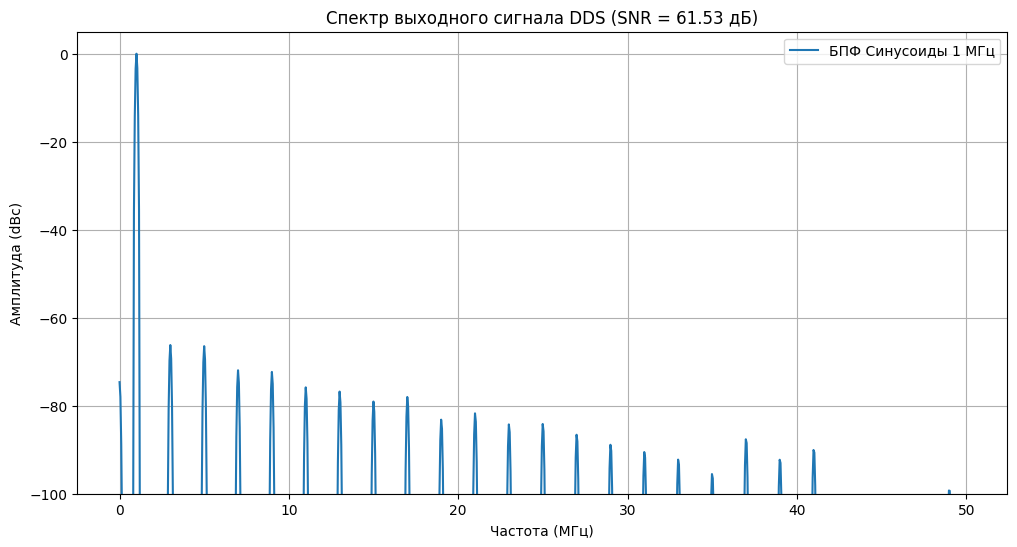
\includegraphics[width=0.9\linewidth]{./assets/sfdr_examp.png}
    \caption{Появление ошибки по фазе при усечении младших битов фазового аккумулятора}
    \label{fig:phase_error}
\end{figure}

Поэтому используется только часть бит фазового аккумулятора, что приводит к появляению ошибки по фазе, пример представлен на рисунке \ref{fig:phase_error}, при отбрасывании младших бит. Эта ошибка приводит к появлению погрешности амплитуды при преобразовании фазы в амплитуду. Такая погрешность является периодической и проявляется в виде побочных спектральных составляющих. На распределение фаз и амплитуд этих составляющих влияют три фактора \cite{spectr}:
\begin{itemize}
    \item разрядность аккумулятора фазы ($A$ бит);
    \item разрядность слова фазы после усчения ($P$ бит);
    \item значение кода частоты ($T$).
\end{itemize}

При некоторых значениях кода частоты составляющие, вызванные усечением, отсутствуют, в то время как при некоторых других значениях эти составляющие имеют максимальный уровень. При $A-P\ge 4$ бит, максимальный уровень паразитных составляющих можно достаточно точно определить как:
\begin{equation} \label{sfdr_approx}
    -6,02\times P\text{ дБ}
\end{equation}
Для 32-разрядного DDS с 12-разрядным кодом фазы максимальный уровень паразитных составляющих будет около $-72$ дБ.

Худшим случаем является ситуация, когда НОД $T$ и $2^{A-P}$ равен $2^{A-P-1}$. Предельный случай, соответствующий отсутствию паразитных составляющих. При этом НОД $T$ и $2^{A-P}$ равен $2^{A-P}$, другими словами, когда в отбрасываемой части кода фазы все разряды равны нулю. Иные значения кода частоты приводят к промежуточным значениям уровня паразитных составляющих, вызванных усечением \cite{spectr}.

Рассматривая паразитные составляющие на качественном уровне, можно сказать, что величина ошибки меняется по пилообразному закону. Для того чтобы вычислить частоту этого сигнала, можно рассмотреть ту часть, которая отбрасывается при усечении аккумулятора фазы. Разрядность этой части равна числу отбрасываемых бит ($B$). Значит, она способна воспринимать только младшую часть кода частоты. Поэтому частота сигнала ошибки будет равна:
\begin{equation}
    f_{error} = f_{clk} \times \frac{ET}{2^B}
\end{equation}
где $f_{clk}$ - частота дискретизации; $ET$ - код частоты, представленный значением отброшенных битов при выполнении усечения.

Для оценки качества сигнала используется метрика $SFDR$ (Spurious Free Dynamic Range) - динамический диапазон без паразитных составляющих. Он определяется как разница в децибелах между уровнем основного сигнала и уровнем самой высокой паразитной составляющей.

\begin{equation} \label{sfdr1}
    SFDR = A_{main} - A_{spur} \text{ дБ}
\end{equation}

\begin{equation} \label{sfdr2}
    SFDR = 20\log_{10}\left(\frac{A_{main}}{A_{spur}}\right)
\end{equation}

\begin{figure}
    \centering
    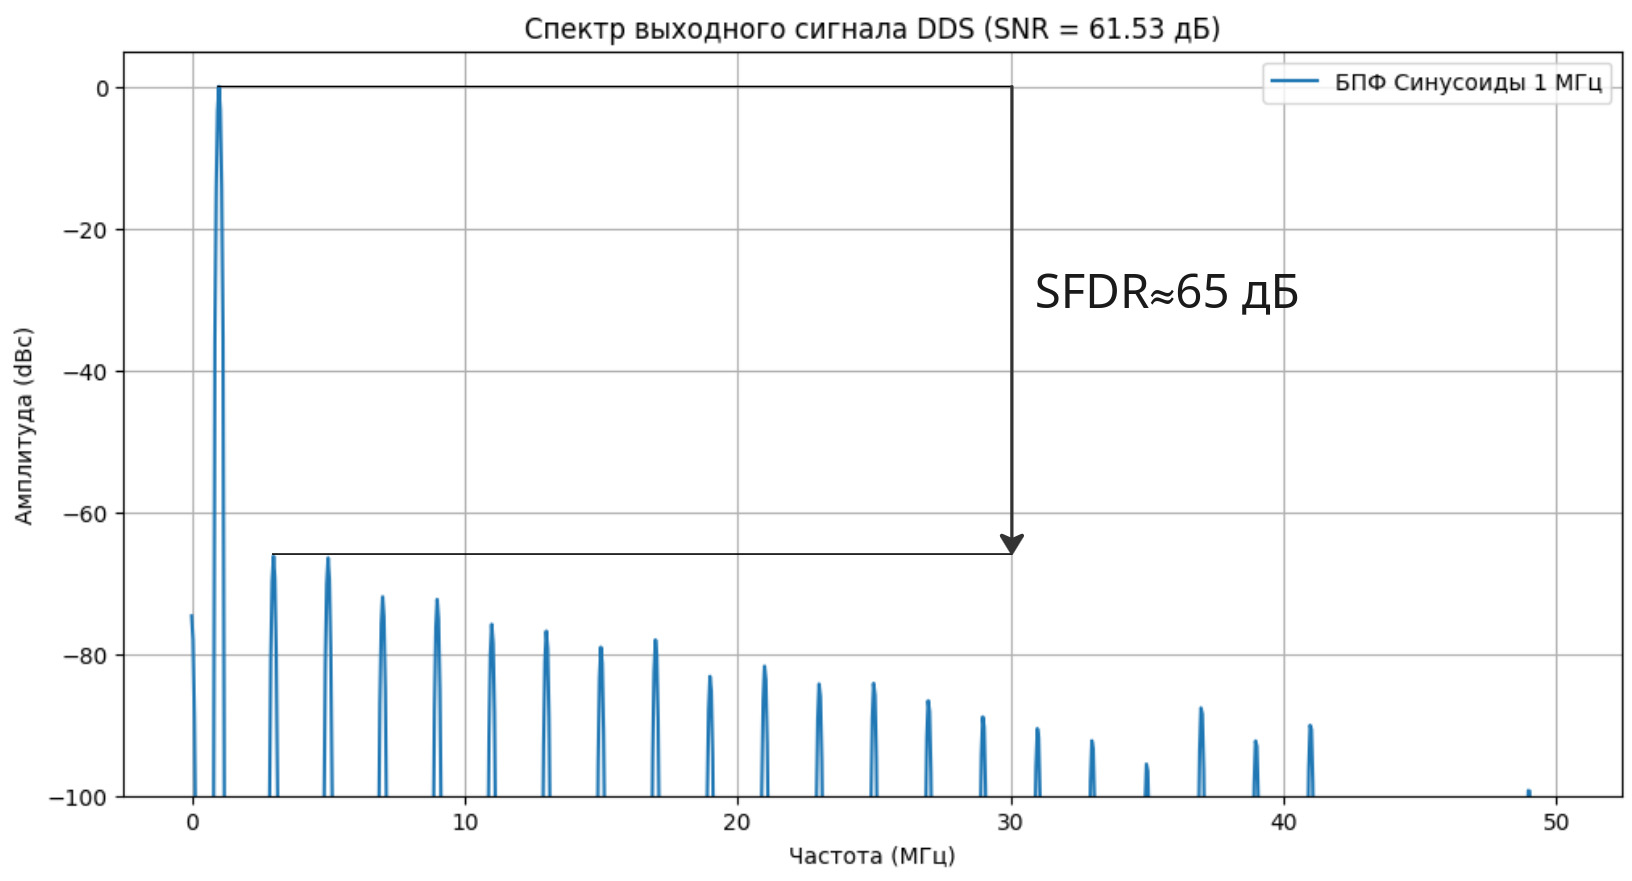
\includegraphics[width=0.9\linewidth]{./assets/sfdr_examp_view.jpg}
    \caption{Пример спектра сигнала, синтезированного с помощью DDS, с паразитными составляющими, вызванными усечением и определением $SFDR$}
    \label{fig:sfdr_example}
\end{figure}

Если принять пик несущей за 0 дБ, то $SFDR$ можно оценить выражением \eqref{sfdr_approx}, что соответствует уровню паразитных составляющих, вызванных усечением. Как представлено на рисунке \ref{fig:sfdr_example}.

\subsection{Сравнение методов CORDIC и DDS}

При выборе метода генерации гармонических сигналов для ГССФ на базе ПЛИС, алгоритм CORDIC и классический DDS с LUT представляют собой два основных подхода.

Выбор конкретного метода зависит от множества факторов, включая требования к функциональности, доступные ресурсы для реализации в ПЛИС, сложность системы и другие требования.

CORDIC и DDS - два кардинально разных метода генерации сигналов, использующие два диаметрально противоположных подхода к формированию выходного сигнала.

Несмотря на математическую эффективность CORDIC алгоритма, в рамках данной работы от его использования было решено отказаться в пользу классического табличного метода с использованием DDS по ряду архитектурных и функциональных причин:

\begin{itemize}
    \item Главным требованием к разрабатываемому ГССФ является возможность генерации не только стандартных периодических сигналов, но и сигналов произвольной формы (Arbitrary Waveforms). Табличный метод естественным образом поддерживает эту функциональность: аккумулятор фазы формирует адрес, по которому из памяти считывается необходимое значение амплитуды. Использование CORDIC, способного вычислять только математически описываемые функции, потребовало бы дополнительной логики для обработки произвольных форм и дополнительного мультиплексирования на выходе.
    \item Исторически алгоритм CORDIC был разработан в условиях жесткого дефицита памяти. Современные ПЛИС обладают значительным объемом высокоскоростной блочной памяти (Block RAM). Реализация четвертьволновой таблицы синуса с высокой точностью требует минимальных затрат BRAM, в то время как CORDIC для достижения аналогичной скорости работы потребляет значительное количество логических ресурсов для реализации сумматоров и промежуточных регистров на каждой стадии конвейера.
    \item Конвейерный CORDIC вносит существенную задержку от момента подачи кода фазы до получения значения амплитуды (порядка $N$ тактов для $N$-битной точности). При использовании встроенной памяти ПЛИС данные считываются с фиксированной задержкой в 1-2 такта, что упрощает временную синхронизацию внутри кристалла и позволяет достичь минимального фазового джиттера.
\end{itemize}

\subsection{Цифро-аналоговое преобразование и фильтрация сигнала}

Как видно из структурной схемы (рисунок \ref{fig:2}), выходным каскадом любого DDS генератора является цифро-аналоговый преобразователь (ЦАП) и, аналоговый фильтр нижних частот (ФНЧ). ПЛИС формирует лишь дискретную последовательность цифровых кодов, которая не может быть напрямую использована как аналоговый сигнал.

\subsubsection{Влияние разрядности ЦАП на шум квантования}

Процесс цифро-аналогового преобразования неизбежно вносит в сигнал специфический шум квантования, обусловленный конечной разрядностью ЦАП $N$. Ошибка квантования $e(t)$ представляет собой разницу между идеальным непрерывным сигналом и его дискретным представлением.

Предполагая, что ошибка квантования является случайной величиной, равномерно распределенной в интервале $\left[-\frac{\Delta}{2}, \frac{\Delta}{2}\right]$, где $\Delta=\frac{V_{ref}}{2^N}$ - шаг квантования, а $V_{ref}$ - опорное напряжение ЦАП, можно определить среднеквадратичное значение напряжения шума квантования $U_n$:
\begin{equation} \label{eq:noise_rms}
U_n = \frac{\Delta}{\sqrt{12}} = \frac{V_{ref}}{2^N \sqrt{12}}
\end{equation}

Эффективное значение напряжения для полномасштабного синусоидального сигнала на выходе составляет $U_s = \frac{V_{ref}}{2\sqrt{2}}$

Теоретическое отношение сигнал/шум (Signal-to-Noise Ratio, SNR) для идеального ЦАП определяется выражением \cite{analog-dds}:
\begin{equation} \label{eq:snr}
    SNR = 20 \log_{10}\left(\frac{U_s}{U_n}\right) = 20 \log_{10}\left(\sqrt{1.5} \cdot 2^N\right) \approx 6.02 \cdot N + 1.76 \text{ (дБ)}
\end{equation}

Уравнение (\ref{eq:snr}) является фундаментальным для проектирования цифровых генераторов: оно показывает, что каждый дополнительный аппаратный разряд ЦАП увеличивает теоретическое SNR примерно на 6 дБ. На практике реальное значение SNR или эффективная разрядность (Effective Number of Bits, ENOB) всегда ниже идеального из-за нелинейных искажений преобразователя, фазового джиттера тактового сигнала и тепловых шумов кристалла \cite{analog-dds}.

\subsubsection{Амплитудно-частотные искажения и восстанавливающий фильтр}

Вследствие дискретной природы синтеза, ЦАП функционирует как экстраполятор нулевого порядка (Zero-Order Hold, ZOH), удерживая уровень выходного напряжения неизменным в течение одного периода тактовой частоты $f_{clk}$. В частотной области это эквивалентно умножению идеального спектра дельта-импульсов на частотную характеристику фиксатора нулевого порядка $H_{ZOH}(f)$ \cite{filipovsky2022}:
\begin{equation} \label{eq:zoh}
    H_{ZOH}(f) = T_{clk} \frac{\sin(\pi f T_{clk})}{\pi f T_{clk}} = \text{sinc}\left(\frac{f}{f_{clk}}\right)
\end{equation}

Наличие множителя $\text{sinc}(x)$ приводит к спаду амплитуды формируемого сигнала с ростом частоты $f_{out}$. В частности, на частоте Найквиста ($f_{out} = \frac{f_{clk}}{2}$) затухание амплитуды основной гармоники составит:
\begin{equation}
20 \log_{10}\left(\frac{\sin(\pi/2)}{\pi/2}\right) = 20 \log_{10}\left(\frac{2}{\pi}\right) \approx -3.92 \text{ дБ}
\end{equation}

Помимо спада амплитуды, спектр ступенчатого сигнала содержит побочные спектральные составляющие (зеркальные частоты), располагающиеся симметрично относительно частоты тактирования и ее гармоник: $k\cdot f_{clk} \pm f_{out}$.

Согласно теореме Котельникова, максимальная синтезируемая частота строго ограничена половиной частоты тактирования ($f_{max} < \frac{f_{clk}}{2}$). На практике для надежного подавления зеркальных компонент максимальную выходную частоту ограничивают на уровне $0.3 \dots 0.4 \cdot f_{clk}$. Для выделения полезного сигнала применяется восстанавливающий аналоговый фильтр нижних частот.

\begin{figure}[htpb]
    \centering
    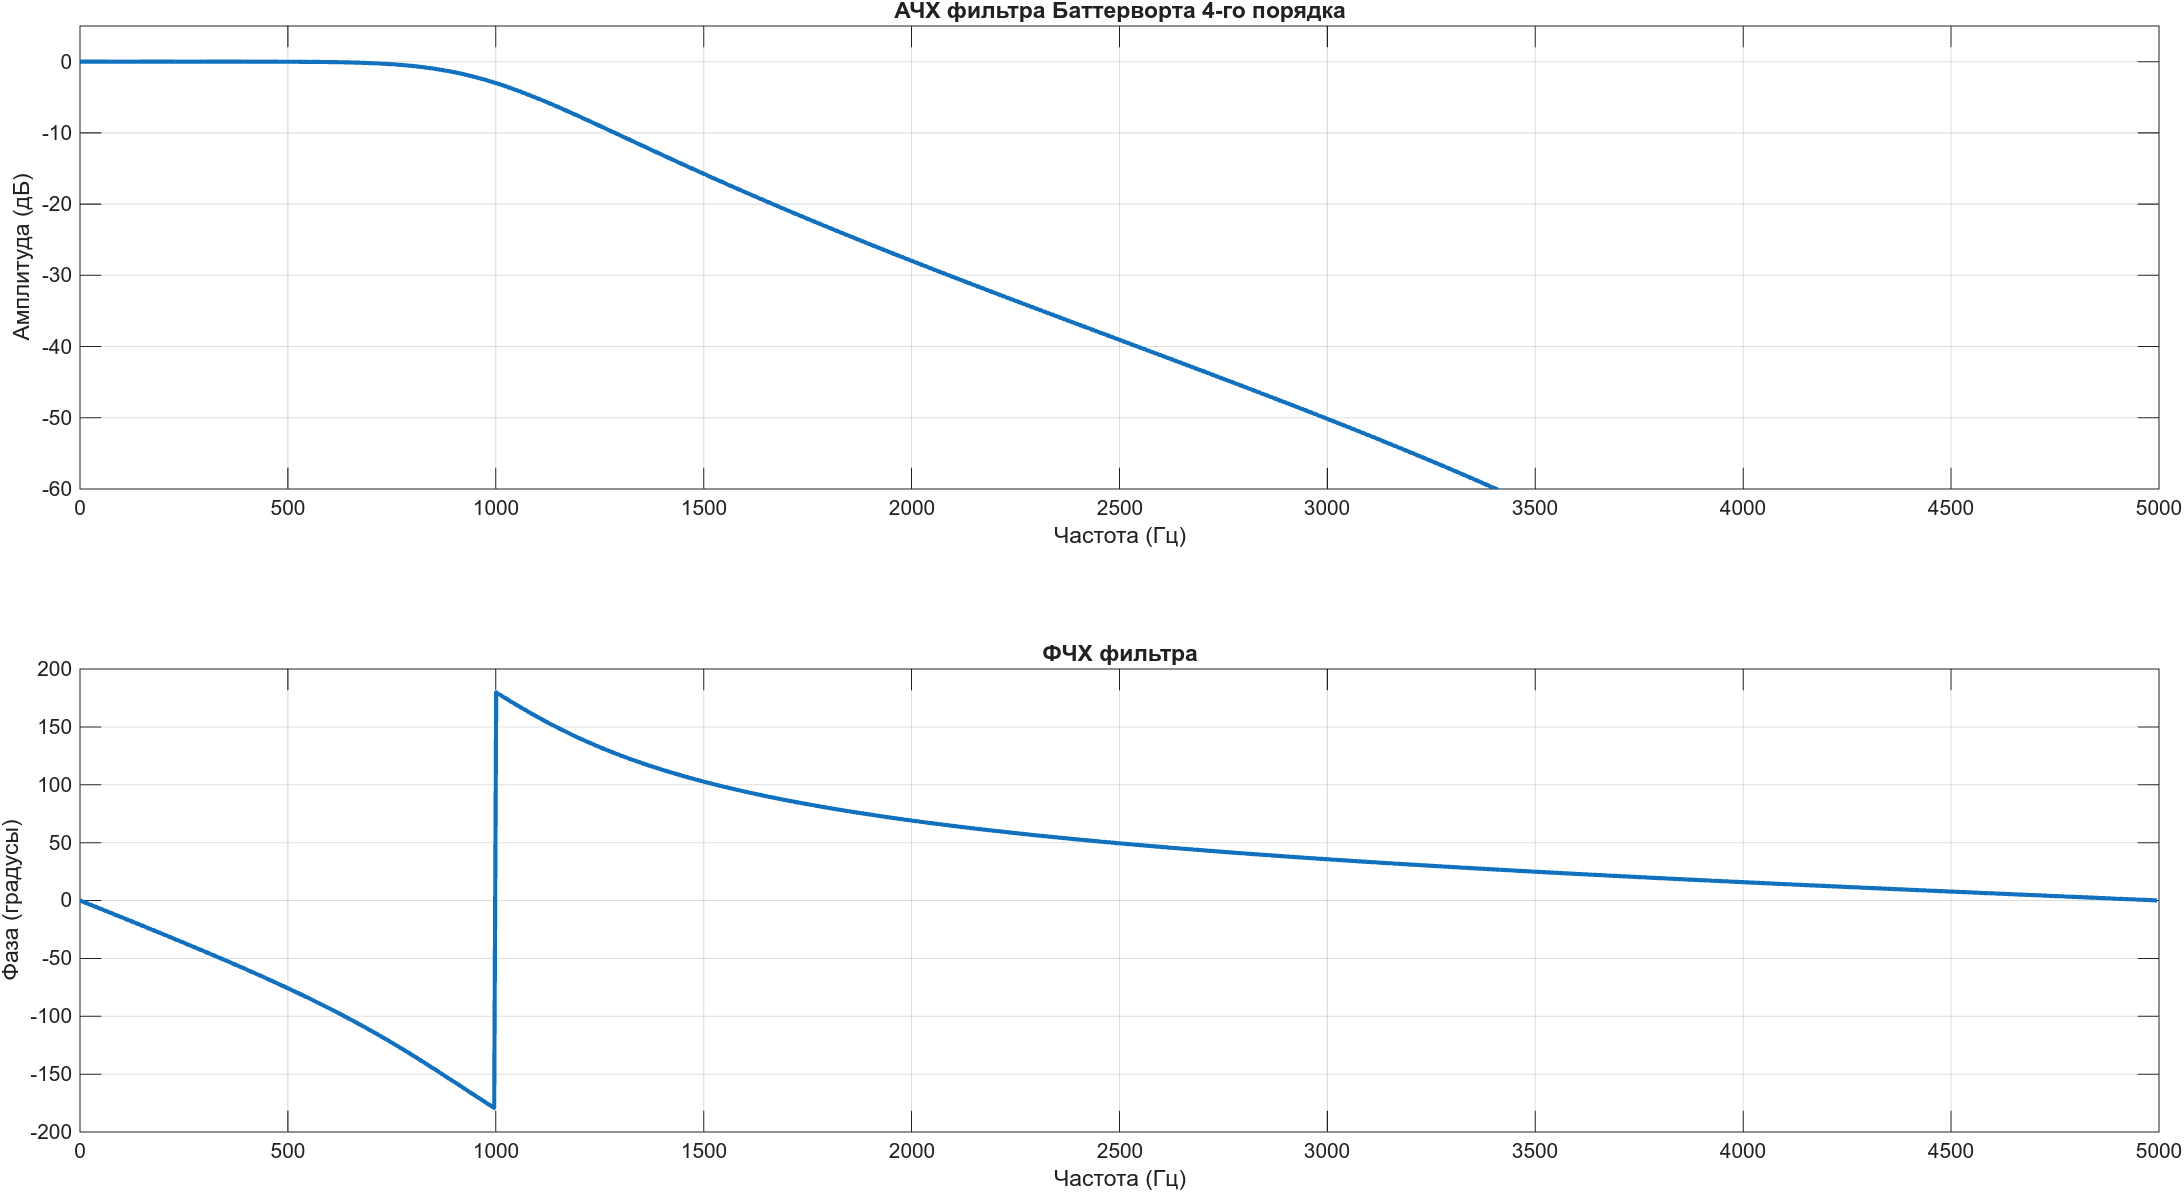
\includegraphics[width=1.0\linewidth]{./assets/Figure_1.png}
    \caption{АЧХ и ФЧХ фильтра Баттерворта 4-го порядка}
    \label{fig:butter}
\end{figure}

Для сохранения стабильной амплитуды генерируемого сигнала в полосе пропускания используют фильтр Баттерворта, обладающий максимально плоской амплитудно-частотной характеристикой \cite{filipovsky2022}. АЧХ и ФЧХ фильтра Баттерворта представлена на рисунок \ref{fig:butter}.

Квадрат модуля передаточной функции фильтра Баттерворта $n$-го порядка имеет вид:
\begin{equation} \label{eq:butterworth}
|H(j\omega)|^2 = \frac{1}{1 + \left(\frac{\omega}{\omega_c}\right)^{2n}}
\end{equation}
где $\omega_c=2\pi f_c$ - круговая частота среза фильтра. Порядок аналогового фильтра $n$ выбирается разработчиком исходя из компромисса между требуемой крутизной спада АЧХ и вносимыми фазовыми искажениями.


\subsection{Обоснование выбора аппаратной платформы}

Реализация ГССФ с заданными характеристиками требует выбора вычислительного базиса, способного обеспечить детерминированность временных интервалов и высокую скорость обработки данных.

Для решения данной задачи рассматривались три класса устройств:
\begin{enumerate}
    \item Микроконтроллеры (MCU): Обладают низкой стоимостью и простотой программирования. Однако программная реализация DDS на MCU ограничена последовательным характером исполнения инструкций. На высоких частотах возникают задержки, вызванные обработкой прерываний и работой системной шины, что недопустимо для прецизионных генераторов \cite{mcu-shit}.
    \item Специализированные ИС прямого цифрового синтеза: Например, микросхемы серии AD9850. Такие устройства обеспечивают высокую чистоту спектра, но в них невозможно реализовать специфические требования \cite{ad9850}.
    \item Программируемые логические интегральные схемы: Сочетают в себе скорость аппаратных решений и гибкость программных систем.
\end{enumerate}

Сравнительный анализ показал, что для реализации ГССФ с возможностью оперативного управления параметрами сигнала наиболее оправданным является использование ПЛИС. В отличие от микроконтроллеров, ПЛИС обеспечивает строго детерминированную аппаратную реализацию каждого этапа синтеза, что исключает фазовый джиттер. В сравнении со специализированными ИС, ПЛИС предоставляет разработчику полную свободу в проектировании архитектуры, позволяя интегрировать блоки управления амплитудой, смещением и скважностью импульсов непосредственно в цифровой тракт.

\section{Разработка архитектуры и программная реализация}

Разработка аппаратной части ГССФ начинается с структурной схемы уровня регистровых передач (RTL). В качестве целевой платформы выбрана ПЛИС семейства Artix-7. Для описания аппаратуры используется язык SystemVerilog.

Архитектура разрабатываемого генератора строится по принципу модульности и включает в себя три основных функциональных области:
\begin{enumerate}
    \item Блок управления и конфигурации, который отвечает за прием внешних управляющих сигналов.
    \item Вычислительное ядро DDS, которое содержит фазовый аккумулятор и преобразователь <<фаза-амплитуда>>, как показано на рисунке \ref{fig:2}.
    \item Контроллер выходного интерфейса, обеспечивающий сериализацию данных и управление внешним ЦАП.
\end{enumerate}

Для обеспечения высокой точности временных интервалов и минимизации фазового шума все основные узлы будут работать в едином тактовом домене. Выходной контроллер реализует SPI протокол, гарантирующий передачу 12-битных отсчетов на микросхему ЦАП.

\subsection{Структурная схема устройства}
Архитектура разрабатываемого генератора строится на базе модуля верхнего уровня (Top-Level), который выполняет интеграцию и маршрутизацию сигналов между всеми функциональными узлами системы. Как показано на рисунке \ref{fig:3}, информационный путь устройства обеспечивает прохождение данных от интерфейса управления до цифро-аналогового преобразователя.

Аппаратная реализация разбита на следующие подсистемы:
\begin{enumerate}
    \item Блок управления и интерфейс связи: реализован на базе IP-ядра Virtual Input/Output (VIO). Обеспечивает управления параметрами генератора с хост-ПК. VIO формирует конфигурационные векторы для ядра DDS (шаг фазы, амплитуда, смещение, скважность и выбор формы сигнала), а также управляет записью пользовательских данных в память (сигналы \texttt{we} , \texttt{addr\_w} и \texttt{data\_in}).
    \item Вычислительное ядро DDS и память (dual\_port\_ram\_awg): центральный узел формирования отсчетов. Ядро DDS рассчитывает текущую фазу и формирует выходной сигнал \texttt{out}. Для режима генерации сигналов произвольной формы (AWG) используется двухпортовая оперативная память. Один порт (запись) асинхронно тактируется сигналами от VIO, второй порт (чтение) синхронизирован с ядром DDS.
    \item Подсистема цифро-аналогового преобразования: отвечает за передачу сформированных отсчетов на внешний ЦАП. Включает в себя:
    \begin{itemize}
        \item \texttt{clk\_divider} - делитель тактовой частоты, формирующий тактовый сигнал 25 МГц для обеспечения корректных временных характеристик интерфейса ЦАП;
        \item \texttt{auto\_updater} - модуль мониторинга, отслеживающий изменения на входе от DDS ядра. При обнаружении изменения формирует сигнал \texttt{update}, который инициирует передачу данных на ЦАП;
        \item \texttt{SPI} - контроллер последовательного периферийного интерфейса, обеспечивающий передачу 12-битных данных на микросхему ЦАП. Реализует стандартный SPI протокол, соответствующий требованиям выбранного ЦАП, включая формирование сигналов \texttt{SCLK}, \texttt{MOSI} и \texttt{CS}.
    \end{itemize}
    \item Система тактирования: обеспечивает синхронизацию всех узлов устройства.
\end{enumerate}

\begin{figure}[htbp]
    \centering
    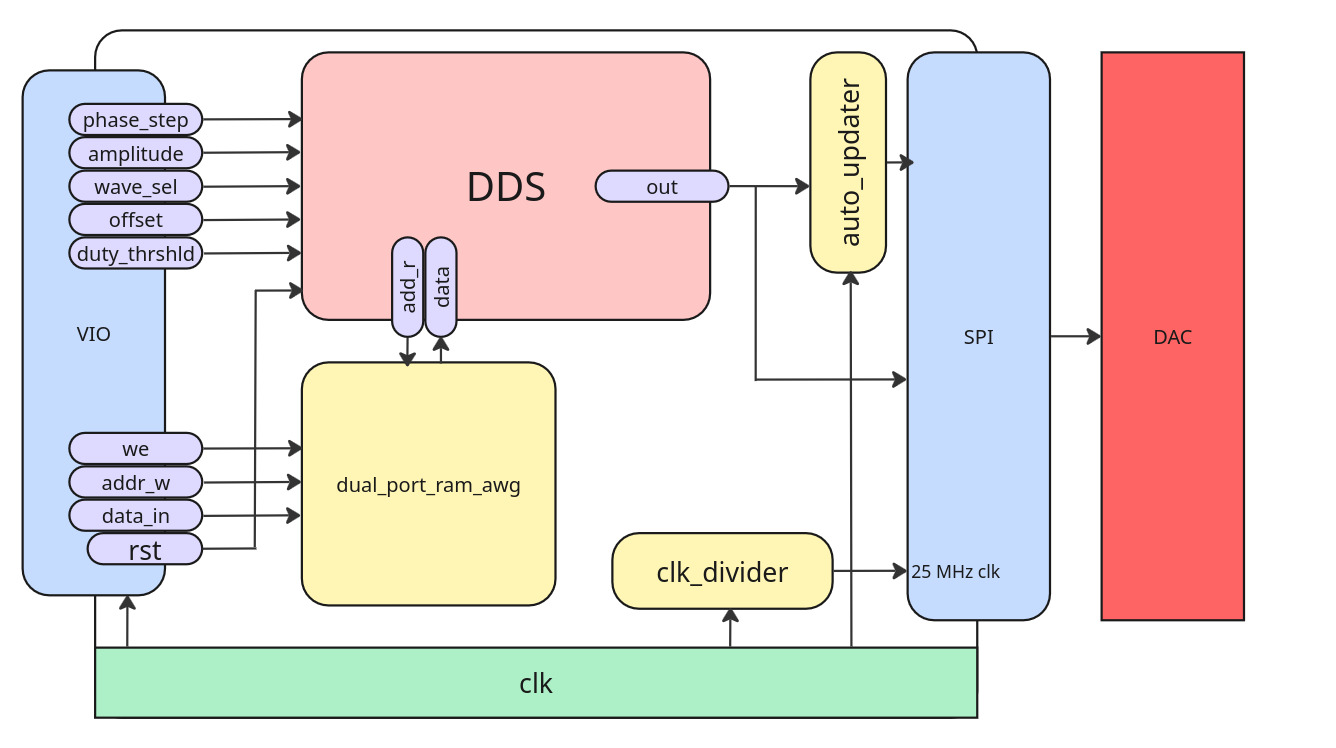
\includegraphics[width=0.93\linewidth]{assets/block-scheme.jpg}
    \caption{Структурная блок-схема ГССФ}
    \label{fig:3}
\end{figure}

\subsection{Проектирование вычислительного ядра DDS}
Вычислительное ядро DDS реализовано в виде строго синхронного конвейерного блока, работающего на частоте $f_{clk}$. Использование конвейерной архитектуры позволяет достичь максимальной пропускной способности - формирование одного нового отсчета сигнала на каждом такте, несмотря на общую задержку вычислений в несколько тактов.

Логику работы ядра можно разделить на три функциональных этапа: накопление фазы, преобразование фазы в амплитуду и цифровая постобработка сигнала.

\subsubsection{Накопление и усечение фазы}
Первым каскадом конвейера является фазовый аккумулятор, представляющий собой 32-разрядный синхронный сумматор с регистром для хранения значения. На каждом такте к текущему значению регистра прибавляется код приращения фазы \texttt{phase\_step}.

Поскольку прямое использование 32-битного значения фазы для адресации памяти потребовало бы объемов BRAM около 4 Гб, в проекте применяется метод усечения фазы. Из полных 32 бит аккумулятора используются только 12 старших разрядов для формирования гармонического сигнала ($P=12$). Согласно теоретическому расчету по формуле (\eqref{sfdr_approx}), использование 12-битного адреса фазы ограничивает максимальный уровень паразитных спектральных составляющих, вызванных усечением, на уровне около $-72$ дБ, что является удовлетворительным, для необходимого качества сигнала.

\subsubsection{Формирование базовых и произвольных сигналов}

Как показано на рисунке \ref{fig:dds_gen}, код фазы в нескольких, отличающихся друг от друга, экземплярах поступает на вход блока управления формой. Этот блок параллельно рассчитывает значения для всех доступных режимов генерации.

Для синтеза гармонических колебаний реализован алгоритм QWS. Логика маршрутизации 12 старших бит аккумулятора работает следующим образом:
\begin{itemize}
    \item \textbf{Бит [11] (S):} определяет необходимость инверсии выходной амплитуды.
    \item \textbf{Бит [10] (D):} управляет направлением чтения из памяти.
    \item \textbf{Бит [9:0]:} 10-битная шина адреса, позволяющая адресовать 1024 ячейки памяти, в которой хранятся предвычисленные значения амплитуды сигнала для первой четверти периода.
\end{itemize}

\begin{figure}[htpb]
    \centering
    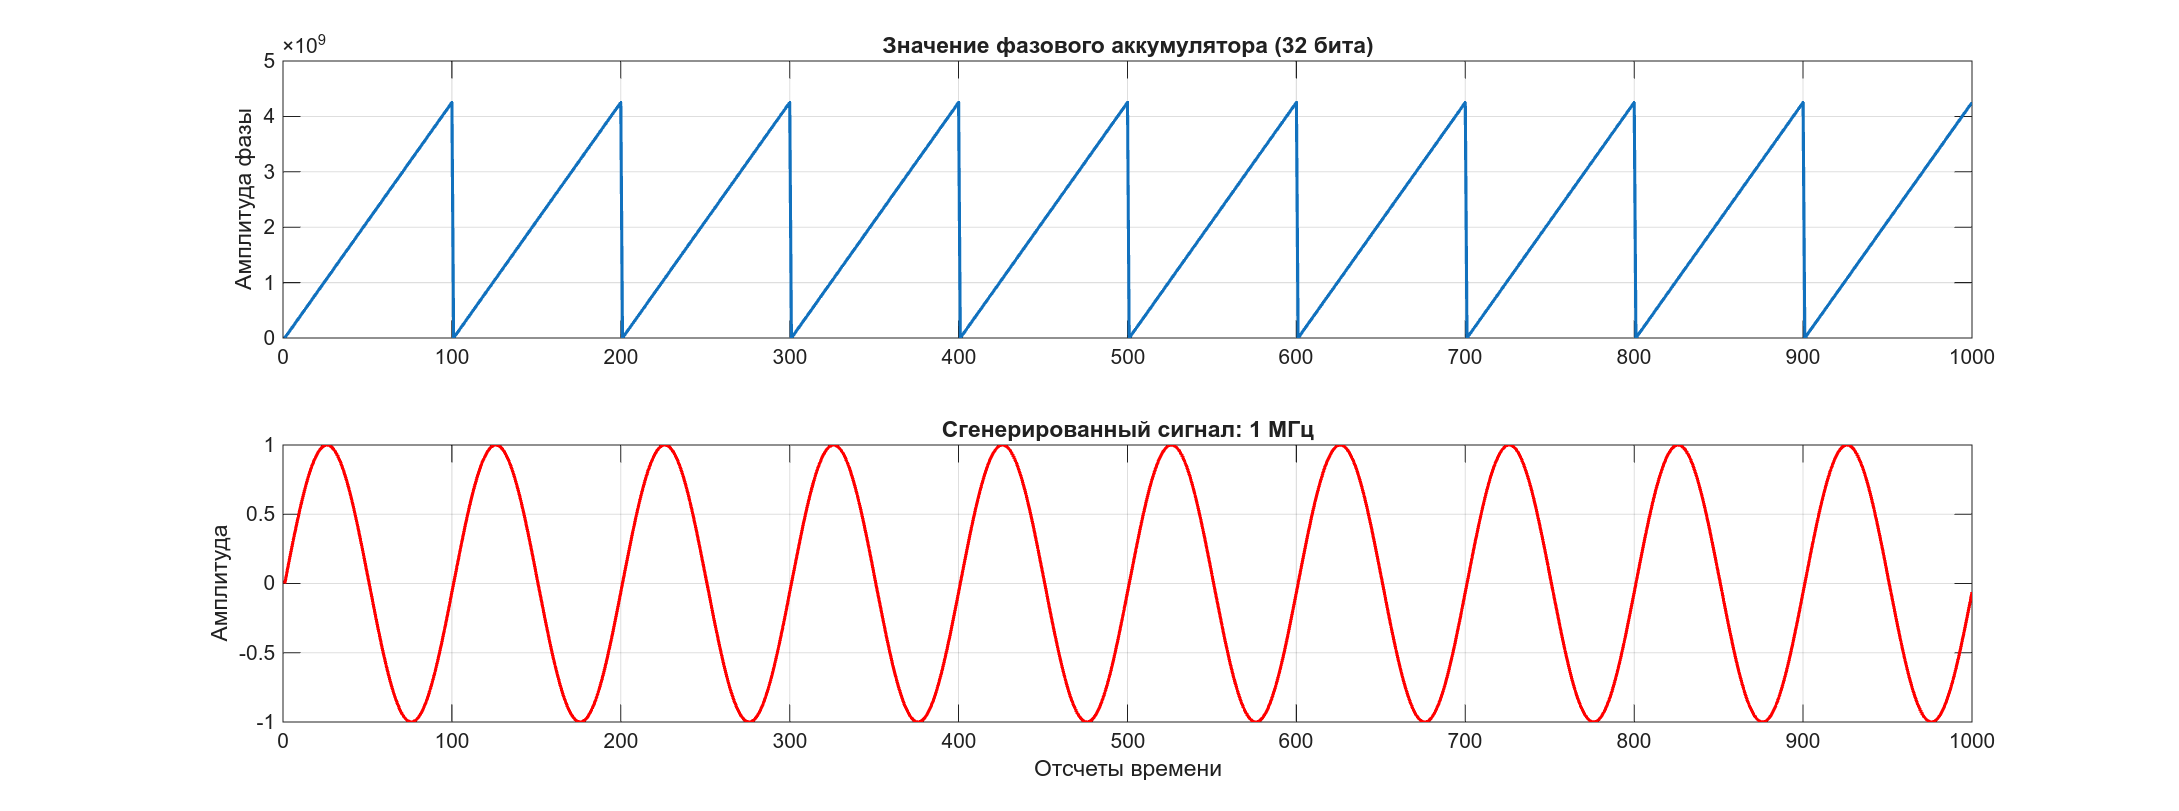
\includegraphics[width=1.0\linewidth]{assets/dds_sim.png}
    \caption{Моделирование работы DDS в режиме генерации гармонических колебаний}
    \label{fig:dds_sim}
\end{figure}

На рисунок \ref{fig:dds_sim} представлен результат моделирования работы DDS генератора в режиме синтеза гармонических колебаний. На рисунке видно, как происходит инкрементирование фазового аккумулятора и его последующее переполнение в конце периода синусоиды.

Как показано на рисунок \ref{fig:dds_gen}, для генерации произвольной формы сигнала предусмотрена встроенная двухпортовая блочная память ПЛИС. В этом режиме 12 старших разрядов аккумулятора фазы используются как линейный счетчик адреса. Это позволяет последовательно считывать все 4096 пользовательских отсчетов.

Стандартные формы сигналов (пилообразный, треугольный и прямоугольный) вычисляются комбинационно. Например, пилообразный сигнал формируется путем прямой передачи 12 старших разрядов аккумулятора на выход мультиплексора. Прямоугольный сигнал формируется цифровым компаратором, сравнивающим значение аккумулятора с заданным порогом скважности \texttt{duty\_threshold}.

Поскольку, чтение данных из BRAM (режим генерации синусоиды и AWG) требует 2 такта синхронизации, а генерация других форм сигнала происходит комбинационно, необходимо использовать сдвиговые выравнивающие регистры. Выравнивающие регистры принудительно задерживают сигналы, сгенерированные комбинационно на 2 такта, чтобы мультиплексор \texttt{wave\_sel} переключался строго синхронные данные.

\subsubsection{Цифровая обработка сигнала (DSP) и защита от переполнения}

После того как мультиплексор выбрал требуемый цифровой код необработанного отсчета, сигнал поступает в блок DSP. Данный каскад отвечает за применение пользовательских настроек амплитуды и смещения постоянной составляющей. Структурная схема конвейера обработки представлена на рисунке \ref{fig:dds_proc}.

Для эффективного использования ресурсов ПЛИС Artix-7, операции масштабирования амплитуды реализованы с применением специализированной аппаратной ячейки DSP48E1, а не на базовых логических элементах. Блоки DSP48E1 аппаратно реализуют функцию $P=A \times B + C$ \cite{dsp48e1}, что подходит для реализации алгоритма работы выходного каскада. Структурная схема аппаратного макроблока DSP48E1, иллюстрирующая путь прохождения данных представлена на рисунок \ref{fig:dsp48e1}. Использование выделенных аппаратных умножителей и сумматоров внутри DSP-слайса освобождает ресурсы базовой логики и значительно повышает максимально достижимую тактовую частоту конвейера.

\begin{figure}[htpb]
    \centering
    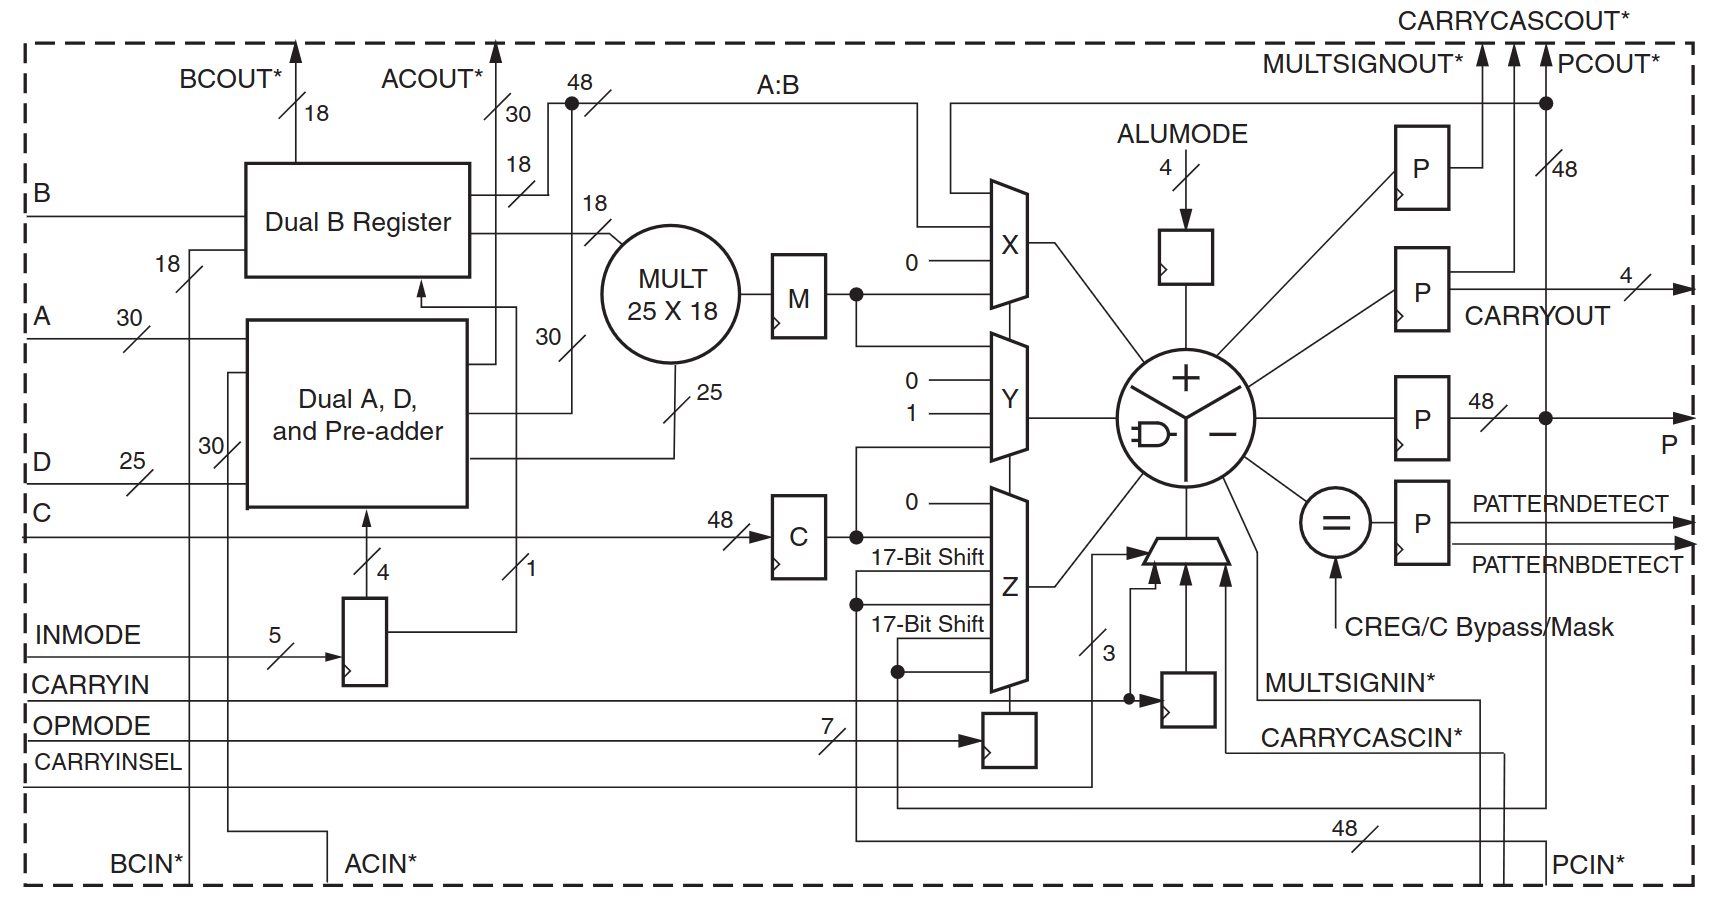
\includegraphics[width=1.0\linewidth]{assets/dsp48e1_scheme.png}
    \caption{Сруктурная схема блока DSP48E1 \cite{dsp48e1}}
    \label{fig:dsp48e1}
\end{figure}

Конвейер DSP состоит из трех стадий:

\begin{enumerate}
    \item \textbf{Буферизация (1 такт):} Фиксация выходного операнда и коэффициентов амплитуды и смещения для обеспечения стабильности сигналов перед математическим преобразованием.
    \item \textbf{Умножение (1 такт):} Перемножение отсчета сигнала на коэффициент амплитуды внутри умножителя DSP-блока.
    \item \textbf{Суммирование и сатурация (1 такт):} Добавление константы смещения \texttt{offset} и проверка выхода за допустимые пределы.
\end{enumerate}

\textbf{Алгоритм сатурации:} Поскольку итоговый сигнал должен быть передан на 12-битный ЦАП, выходное значение ограничено диапазоном от $0$ до $4095$. Если сумма масштабированной амплитуды и смещения превышает значение $4095$, блок сатурации принудительно устанавливает выход в максимальное значение. Аналогично, если результат уходит в отрицательную область, выход фиксируется на нуле. Эта защита надежно предотвращает целочисленное переполнение, исключая возникновение резких фазовых инверсий и деструктивных выбросов на аналоговом выходе.

Для аппаратной реализации алгоритма сатурации используется следующая логика на языке SystemVerilog, предотвращающая целочисленное переполнение:

\begin{lstlisting}[language=Verilog, caption={Реализация алгоритма сатурации амплитуды}]
if (dsp_s3_sum_wide > $signed({2'b0, MAX_VAL})) begin
    bus.dds_out <= MAX_VAL;
end else if (dsp_s3_sum_wide < $signed({2'b11, MIN_VAL[OUT_W-2:0]})) begin
    bus.dds_out <= MIN_VAL;    
end else begin
    bus.dds_out <= dsp_s3_sum_wide[OUT_W-1:0];
end
\end{lstlisting}

Таким образом, общая латентность вычислительного ядра от момента изменения кода частоты до появления нового отсчета на выходе DSP составляет 5 тактов (2 такта BRAM + 3 такта DSP). В контексте непрерывной генерации эта задержка не влияет на частоту выходного сигнала, так как архитектура обеспечивает пропускную способность в один отсчет за каждый такт системной частоты $f_{clk}$.

\begin{figure}[htp]
    \centering
    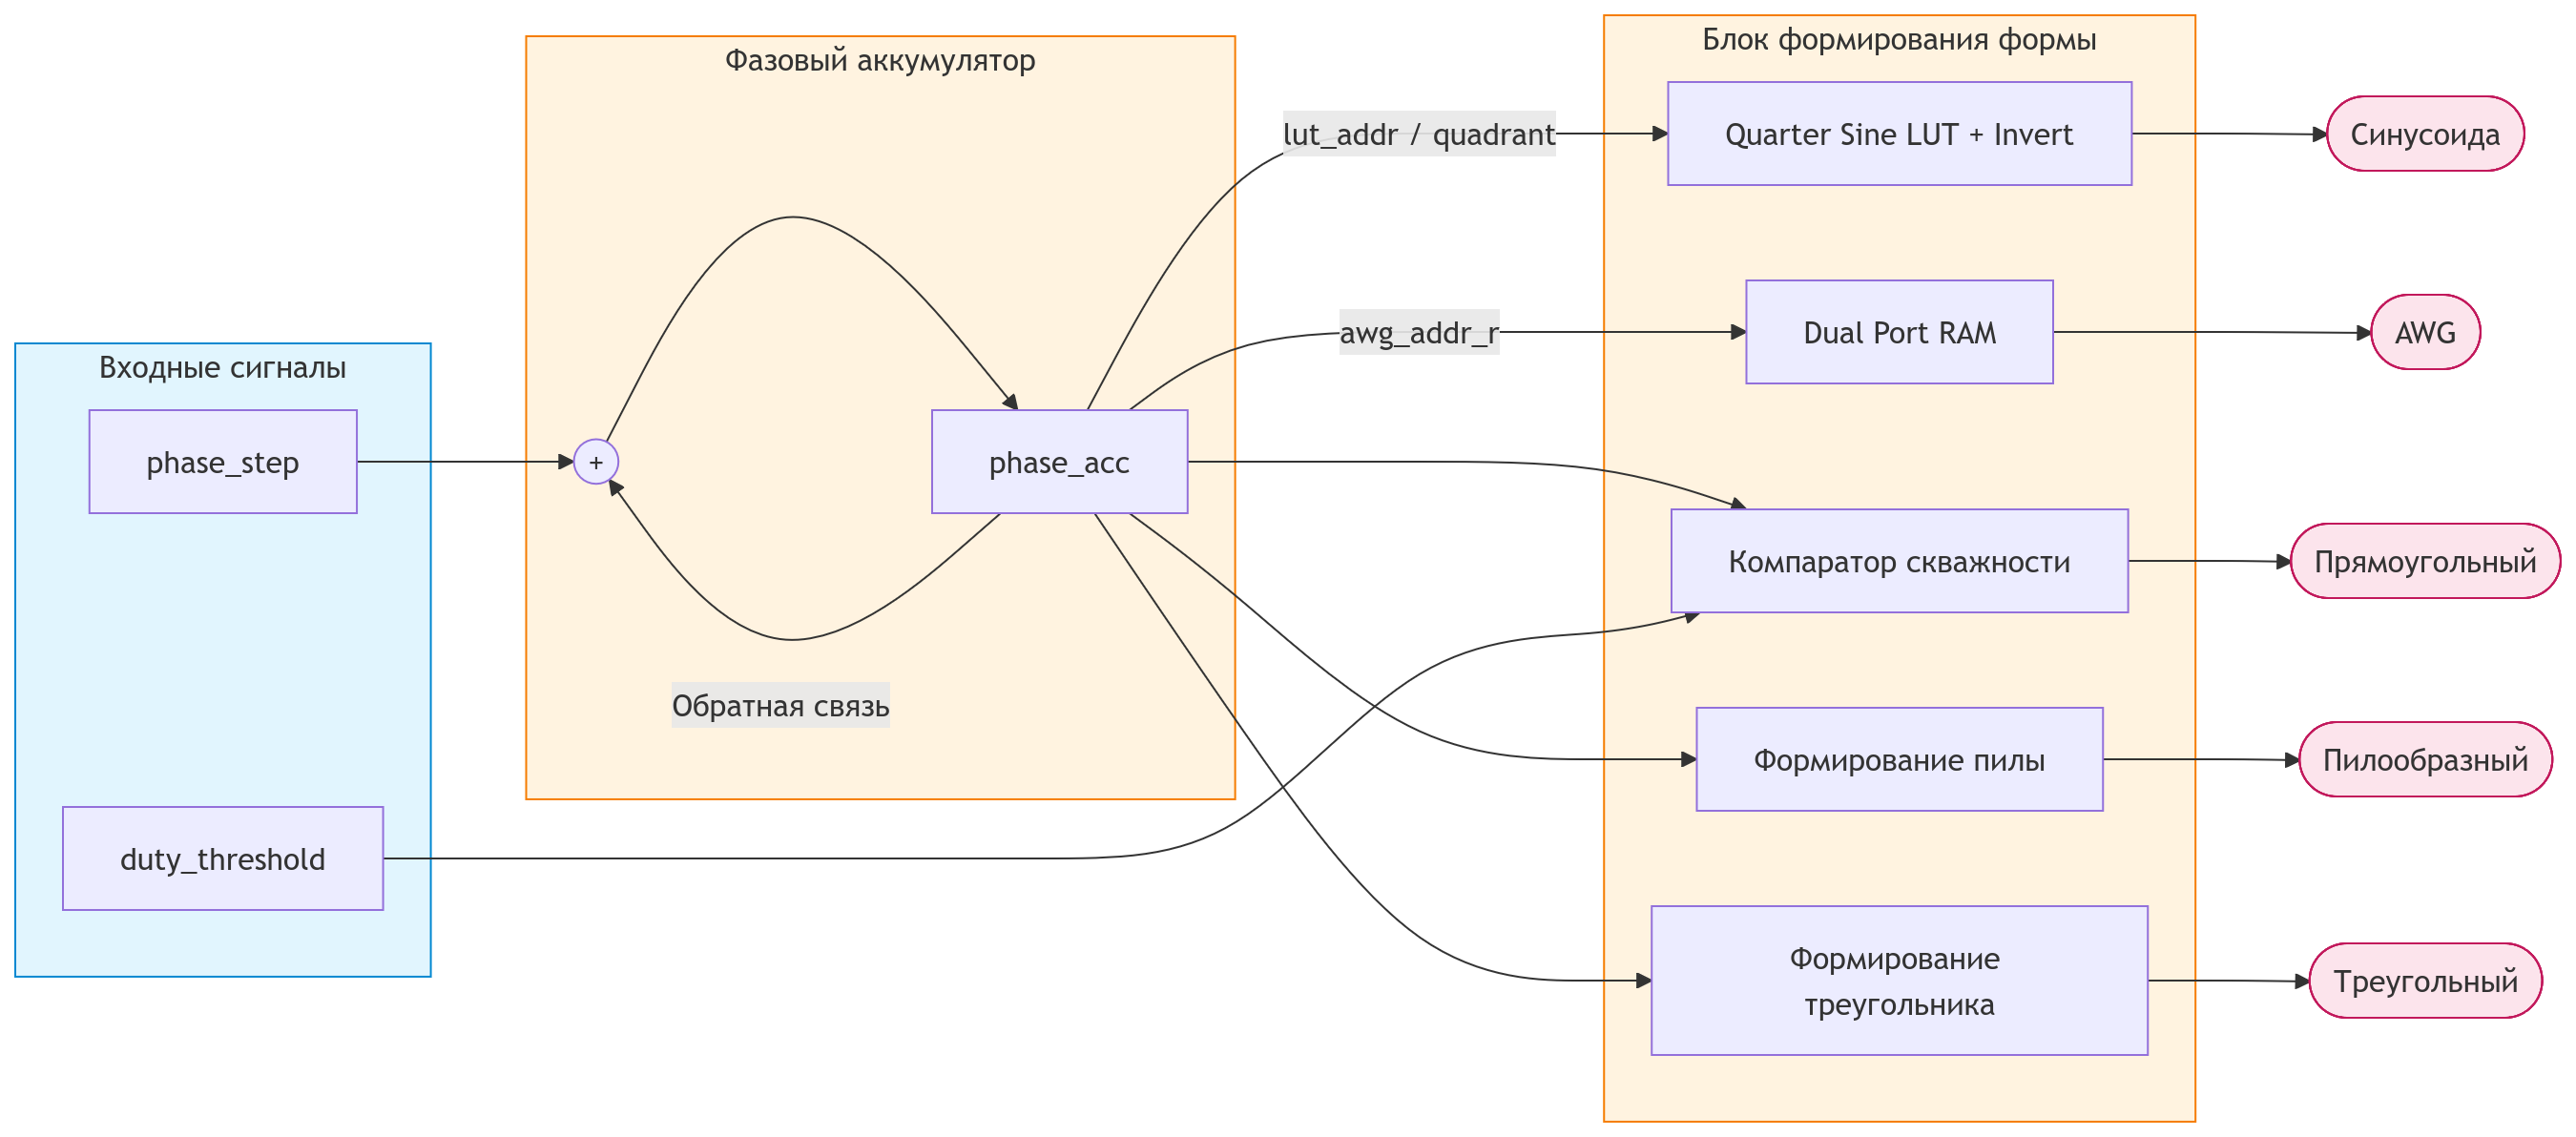
\includegraphics[width=1\linewidth]{assets/dds_gen.png}
    \caption{Структурная схема генерации необработанных отсчетов сигнала}
    \label{fig:dds_gen}
\end{figure}

\begin{figure}[htp]
    \centering
    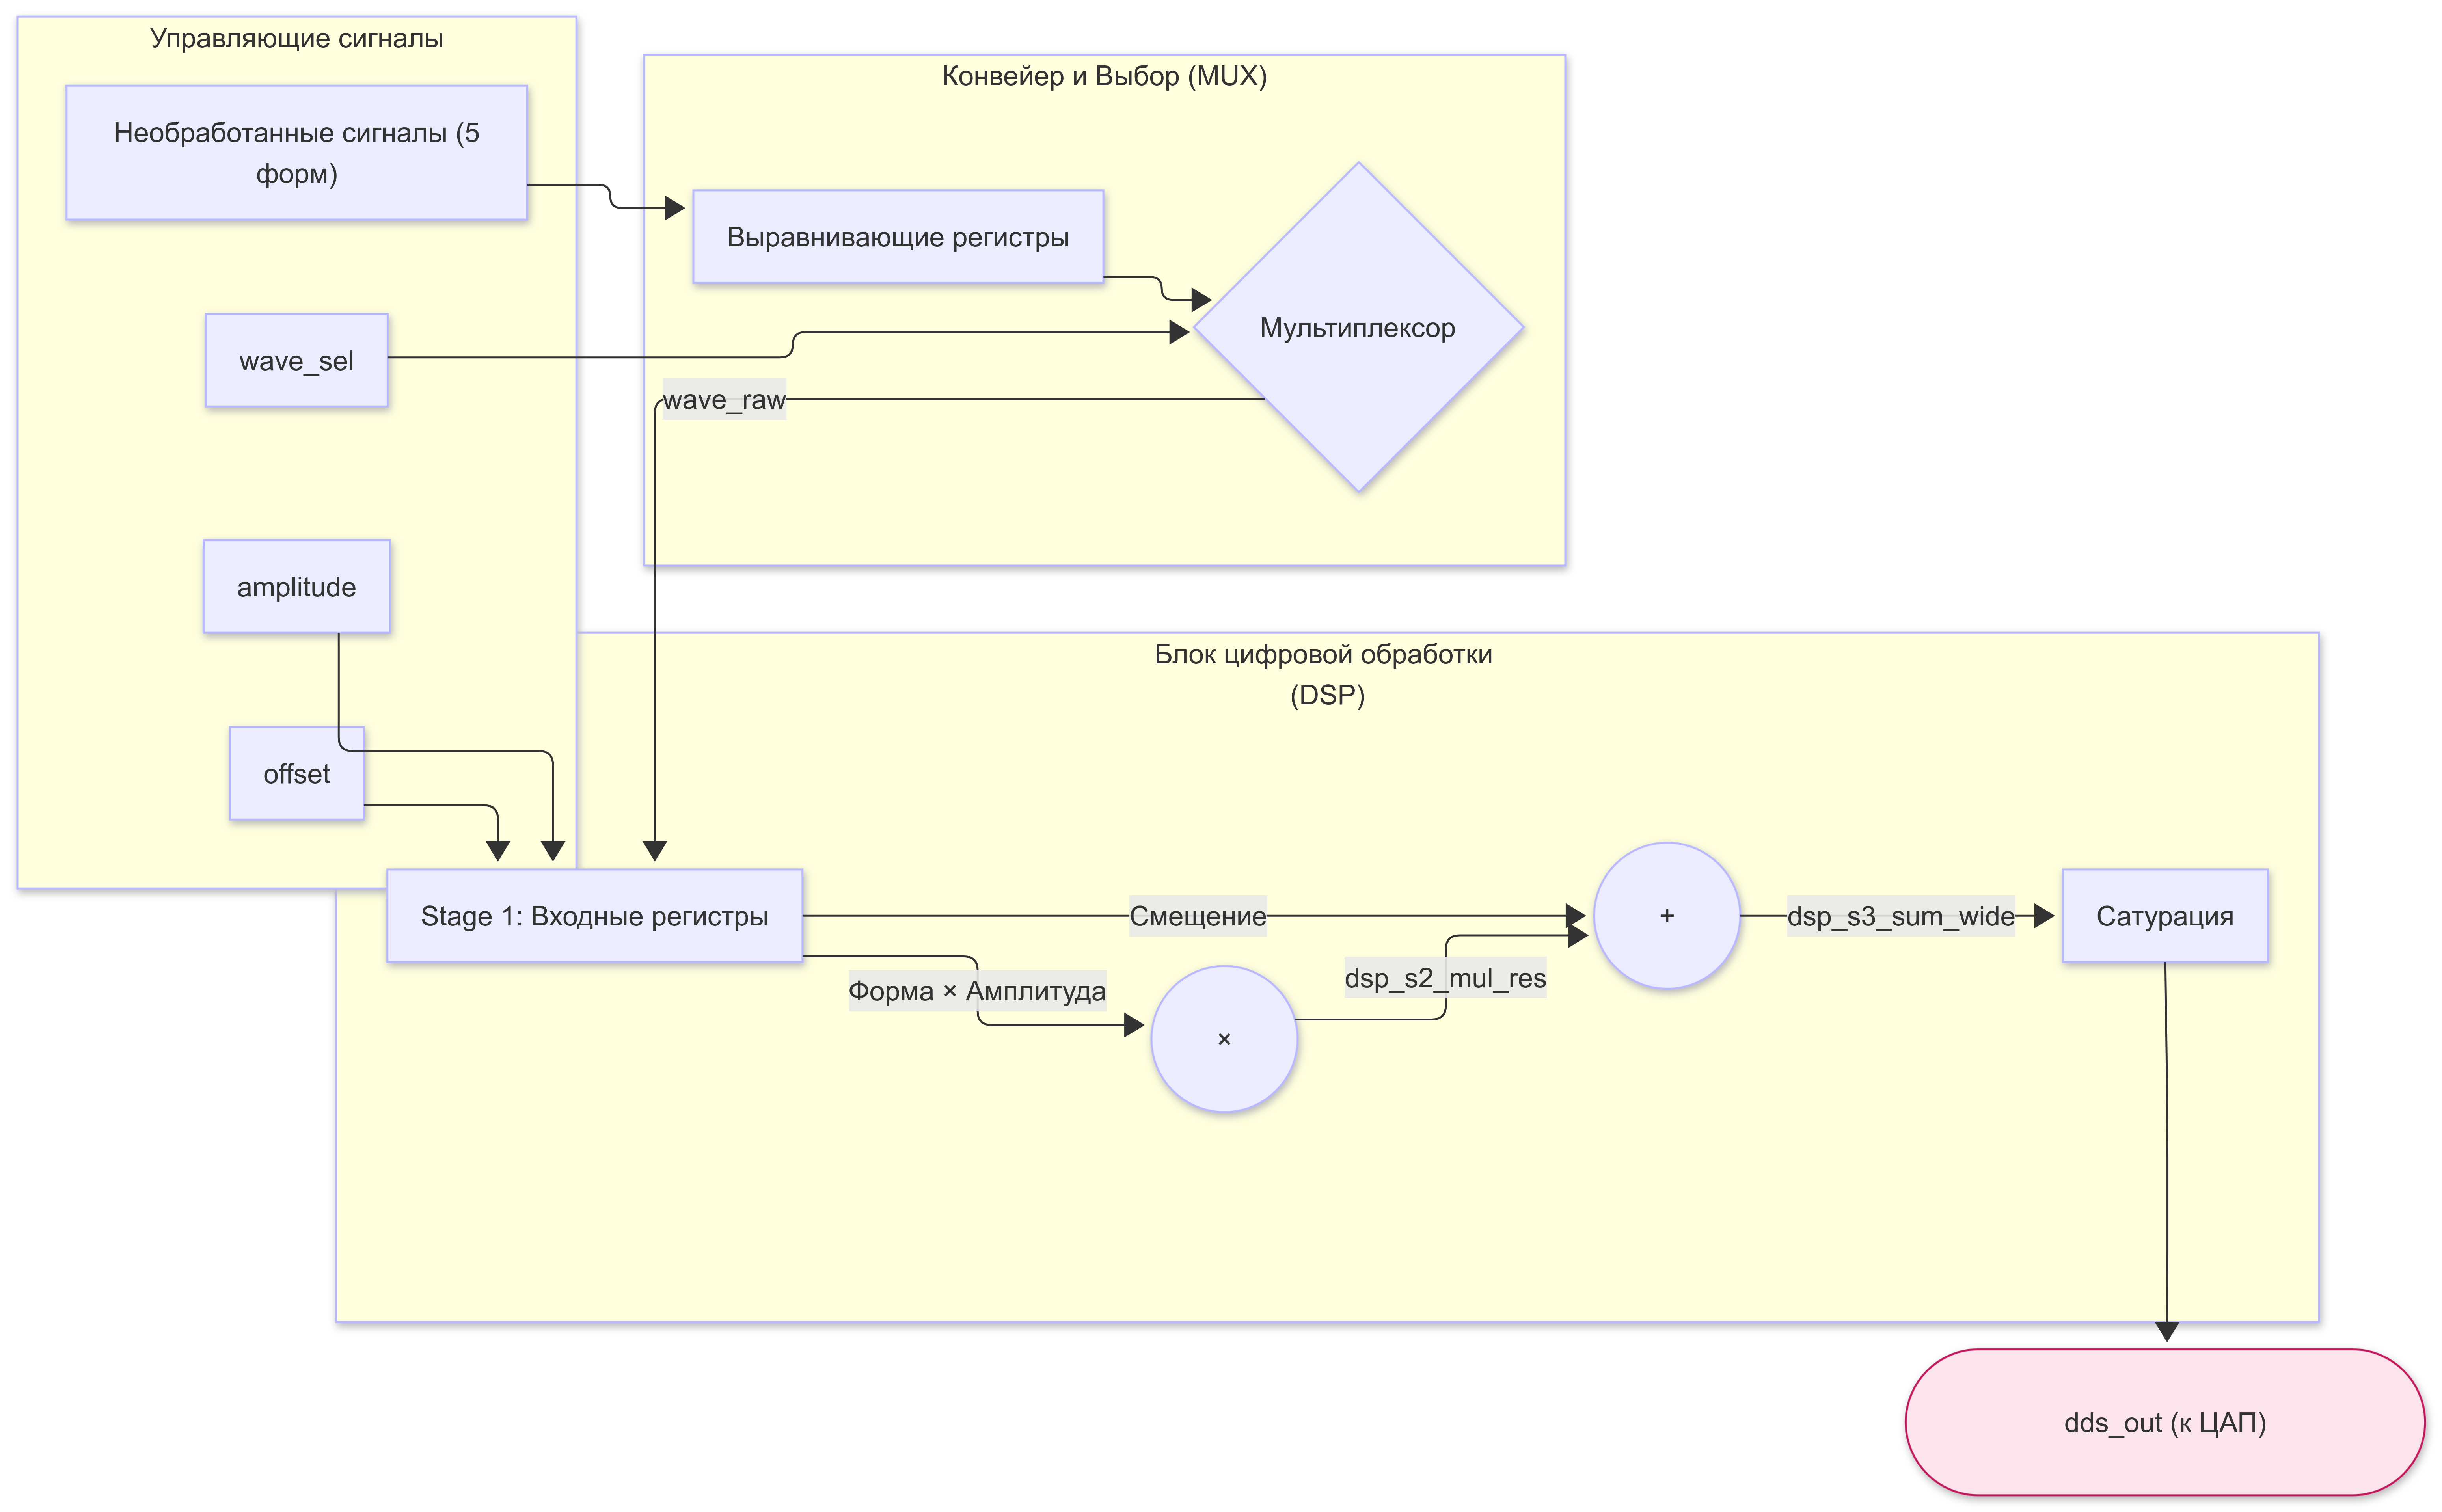
\includegraphics[width=1\linewidth]{assets/dsp1.png} 
    \caption{Структурная схема конвейера и цифровой обработки (DSP)}
    \label{fig:dds_proc}
\end{figure}

\subsection{Разработка контроллера цифро-аналогового преобразователя}

Вычислительное ядро DDS формирует параллельные 12-битные отсчеты амплитуды сигнала. Однако для аналогового воспроизведения этого сигнала требуется передача данных на внешний ЦАП, представленный модулем PmodDA2.

Микросхема ЦАП использует синхронный последовательный интерфейс SPI. В связи с этим возникает необходимость в разработке контроллера, который будет сериализовать параллельные данные и формировать сигналы управления:
\begin{itemize}
    \item \texttt{SYNC} - сигнал выбора кристалла и кадрирования пакета данных;
    \item \texttt{SCLK} - тактовый сигнал последовательного интерфейса;
    \item \texttt{DIN} - линия передачи последовательных данных.
\end{itemize}

Особое внимание при проектировании выходного каскада было уделено проблеме пересечения тактовых доменов (Clock Domain Crossing, CDC). Вычислительное ядро DDS функционирует на высокой системной частоте $f_{clk}$ (100 МГц) для обеспечения максимальной пропускной способности конвейера, в то время как контроллер SPI тактируется частотой 25 МГц, обусловленной аппаратными ограничениями микросхемы DAC121S101 \cite{dac121s101}.

Прямая передача многобитных шин данных между асинхронными тактовыми доменами недопустима, так как может привести к возникновению метастабильности в регистрах и нарушению целостности передаваемого слова амплитуды. Для безопасной передачи 12-битных отсчетов из домена $f_{clk}$ в домен SPI применяется механизм рукопожатия с использованием регистров-синхронизаторов. 

Сигнал готовности новых данных \texttt{updateData}, формируемый в ядре DDS, проходит через двухтриггерный синхронизатор в тактовом домене SPI контроллера. Только после успешной синхронизации флага валидности, конечный автомат захватывает параллельный код амплитуды в свой внутренний сдвиговый регистр, что гарантирует стабильность данных на момент их защелкивания и исключает риск метастабильности.

Для управления процессом передачи разработан контроллер, логика работы которого построена на базе конечного автомата (FSM). Автомат имеет два основных состояния: \texttt{IDLE} (ожидание) и \texttt{UPDATE} (передача данных). Переход в активное состояние инициируется внутренним сигналом \texttt{updateData}, который формируется синхронно с обновлением отсчета в ядре DDS.

Pmod DA2 построен на базе микросхемы DAC121S101. Согласно технической спецификации \cite{dac121s101} на микросхему DAC121S101 формат коммуникационной посылки состоит из 16 бит. Четыре старших бита отвечают за конфигурацию режимов энергопотребления (в штатном режиме передаются нули), а 12 младших бит содержат полезную нагрузку — цифровой код амплитуды.

Алгоритм работы контроллера следующий:
\begin{enumerate}
    \item При получении сигнала \texttt{updateData} FSM переходит в состояние \texttt{UPDATE} и устанеавливает линию \texttt{SYNC} в логический ноль, сигнализируя начало передачи.
    \item Данные из ядра DDS защелкиваются во внутреннем сдвиговом регистре контроллера.
    \item По каждому фронту внешнего тактового сигнала \texttt{ext\_spi\_clk} происходит выдача старшего бита (MSB) из сдвигового регистра на линию \texttt{DIN}.
    \item После передачи всех бит кадра внутренний счетчик \texttt{counter} формирует флаг завершения \texttt{countDone}. Конечный автомат возвращается в состояние \texttt{IDLE}, а линия \texttt{SYNC} возвращается в высокий уровень, завершая цикл обновления аналогового выхода.
\end{enumerate}

Реализованный аппаратный контроллер позволяет использовать весь потенциал интерфейса Pmod DA2, обеспечивая надежное обновление выходного напряжения.

\subsection{Верификация RTL-модели и функциональное моделирование}

Перед этапом логического синтеза и имплементации проекта в ПЛИС была проведена функциональная верификация разработанной RTL-модели. Моделирование выполнялось в среде Siemens EDA Questa Advanced Simulator. Данный инструмент обеспечивает высокую точность симуляции и полную поддержку стандартов SystemVerilog.

Для проверки корректности работы устройства был разработан испытательный стенд (testbench), на языке SystemVerilog. Стенд генерирует тактовый сигнал, формирует последовательность сброса и эмулирует подачу управляющих воздействий. Временные ряды выходных сигналов экспортировались в формате CSV. Для обеспечения высокой наглядности и удобства анализа, последующая обработка и визуализация данных выполнялась в Python.

Для обеспечения всестороннего покрытия функционала генератора, помимо базовых направленных тестов (directed tests), была применена методология псевдослучайного тестирования с ограничениями (Constrained Random Testing, CRT). Использование возможностей объектно-ориентированного программирования (ООП), встроенных в стандарт SystemVerilog, позволило создать гибкое и масштабируемое тестовое окружение, следующее методологии CRT.

Структура верификационного окружения включает в себя классы-транзакции, описывающие конфигурационные векторы. Для автоматизированной генерации тестовых воздействий использовался механизм рандомизации с ограничениями (\texttt{randomize() with \{...\} }). Это позволило сгенерировать тысячи уникальных комбинаций входных параметров, исключая при этом логически невозможные или запрещенные состояния системы.

Структурная схема разработанного верификационного окружения представлена на рисунке \ref{fig:tb_arch}.

\begin{figure}[htpb]
    \centering
    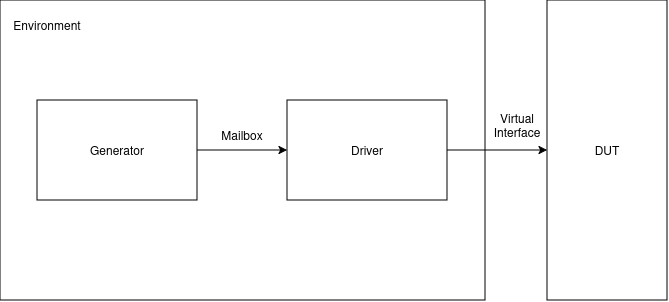
\includegraphics[width=0.8\linewidth]{assets/TB arch.png}
    \caption{Структурная схема объектно-ориентированного тестового стенда}
    \label{fig:tb_arch}
\end{figure}

Архитектура стенда логически разделена на следующие компоненты:
\begin{itemize}
    \item Transaction (\texttt{SignalItem}) — базовый класс данных, инкапсулирующий в себе набор входных параметров (тип сигнала, частота, амплитуда, смещение, скважность) для одного тестового воздействия.
    \item Generator (\texttt{Generator}) — компонент, отвечающий за создание объектов транзакций и их автоматическую рандомизацию на основе математических ограничений (Constraints). Сгенерированные транзакции передаются далее через потокобезопасный канал связи (Mailbox).
    \item Driver (\texttt{Driver}) — компонент нижнего уровня, который извлекает абстрактные транзакции из почтового ящика, производит расчет физических параметров (например, инкремента фазы) и транслирует их в тактовые сигналы на контактах проверяемого устройства (DUT) через виртуальный интерфейс (\texttt{virtual interface}).
    \item Environment (\texttt{Environment}) — класс верхнего уровня, инкапсулирующий генератор и драйвер. Выполняет маршрутизацию почтовых ящиков, инициализацию виртуальных интерфейсов, а также управляет общим ходом симуляции и подачей сигнала сброса (\texttt{reset}).
\end{itemize}

Ключевым элементом, обеспечивающим эффективность CRT, является класс транзакции с описанными правилами рандомизации. В листинге \ref{lst:sig_item} представлен код конфигурационной транзакции генератора.

\begin{lstlisting}[language=Verilog, caption={Класс транзакции с ограничениями рандомизации}, label={lst:sig_item}]
class SignalItem;
    rand enum {SINE, SQUARE, TRIANGLE, SAW} sig_type;
    rand int frequency;
    rand byte amplitude;
    rand int offset;
    rand int duty_threshold;

    constraint freq_range {
        frequency inside {[100:1000000]};
    }
    constraint amp_limit {
        amplitude > 0;
    }
    constraint offset_limit {
        offset inside {[-8192:8191]};
    }
    constraint duty_c {
        if (sig_type == SQUARE) {
            duty_threshold inside {[1000:2000000000]};
        } else {
            duty_threshold == 0;
        } 
    }
    ...
endclass
\end{lstlisting}

Использование модификатора \texttt{rand} сообщает встроенному решателю симулятора о необходимости генерировать случайные значения для переменных класса. Блоки \texttt{constraint} накладывают жесткие ограничения на пространство решений. Например, ограничение \texttt{duty\_c} гарантирует, что параметр скважности будет сгенерирован только в том случае, если выбран прямоугольный тип сигнала (\texttt{SQUARE}), а ограничение \texttt{freq\_range} ограничивает частоту диапазоном от 100 Гц до 1 МГц. Это позволяет концентрировать тестирование исключительно на валидных состояниях системы.

Преобразование абстрактных параметров в физические сигналы осуществляется в компоненте \texttt{Driver}. Фрагмент кода драйвера представлен в листинге \ref{lst:driver}.

\begin{lstlisting}[language=Verilog, caption={Фрагмент класса Driver}, label={lst:driver}]
task run();
    forever begin
        SignalItem item;
        logic [PHASE_W-1:0] calculated_phase_step;

        gen2drv.get(item);

        calculated_phase_step = (item.frequency * (2.0 ** PHASE_W)) / CLK_FREQ;

        @(posedge vif.clk); // Sync
        vif.amplitude      <= item.amplitude;
        vif.offset         <= item.offset;
        vif.duty_threshold <= item.duty_threshold;
        vif.phase_step     <= calculated_phase_step;
        vif.wave_sel       <= item.sig_type;

        repeat(100) @(posedge vif.clk);
    end
endtask
\end{lstlisting}

В данном фрагменте наглядно продемонстрирован расчет инкремента фазы (\texttt{calculated\_phase\_step}) непосредственно внутри тестового окружения. Это освобождает конфигурационную панель от необходимости передавать сырые коды фазы и позволяет оперировать понятными физическими величинами при написании тестов.

Благодаря применению каналов связи (\texttt{mailbox}) и конструкции \texttt{fork...join\_none} в классе \texttt{Environment}, процессы генерации транзакций и управления интерфейсом выполняются параллельно и асинхронно. Подобная модульная архитектура тестового стенда обеспечила высокую масштабируемость и позволила провести исчерпывающее автоматизированное тестирование всех режимов цифрового вычислительного ядра DDS.

\begin{figure}[htpb]
    \centering
    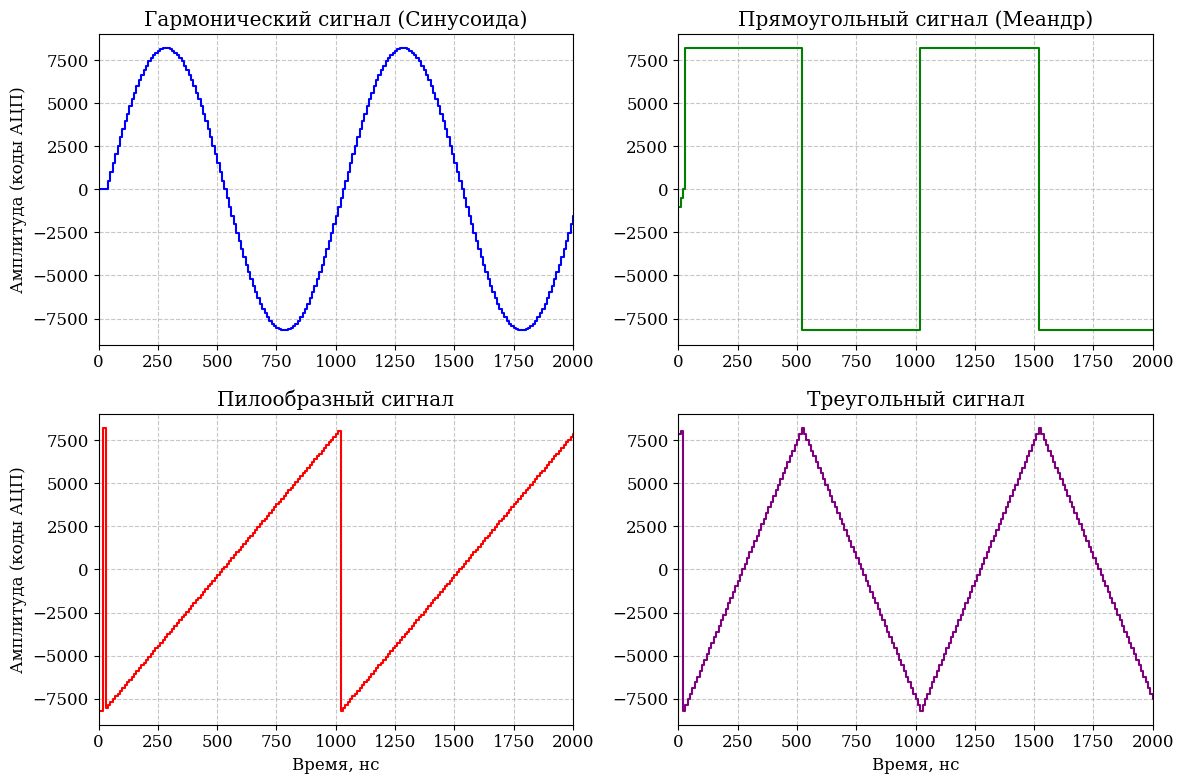
\includegraphics[width=0.9\linewidth]{assets/default_examples.png}
    \caption{Временные диаграммы генерации базовых форм сигналов}
    \label{fig:sim_base_waves}
\end{figure}


Использование ООП-подхода и CRT позволило выявить граничные случаи (corner cases) в работе конвейера DSP и логики усечения фазы, которые могли быть упущены при ручном написании направленных тестов. Автоматизированная система проверки (Scoreboard) сравнивала выходные отсчеты RTL-модели с эталонной программной моделью, написанной на высоком уровне абстракции, что гарантировало побитовую точность работы аппаратного генератора во всем диапазоне допустимых значений.

\begin{figure}[htpb]
    \centering
    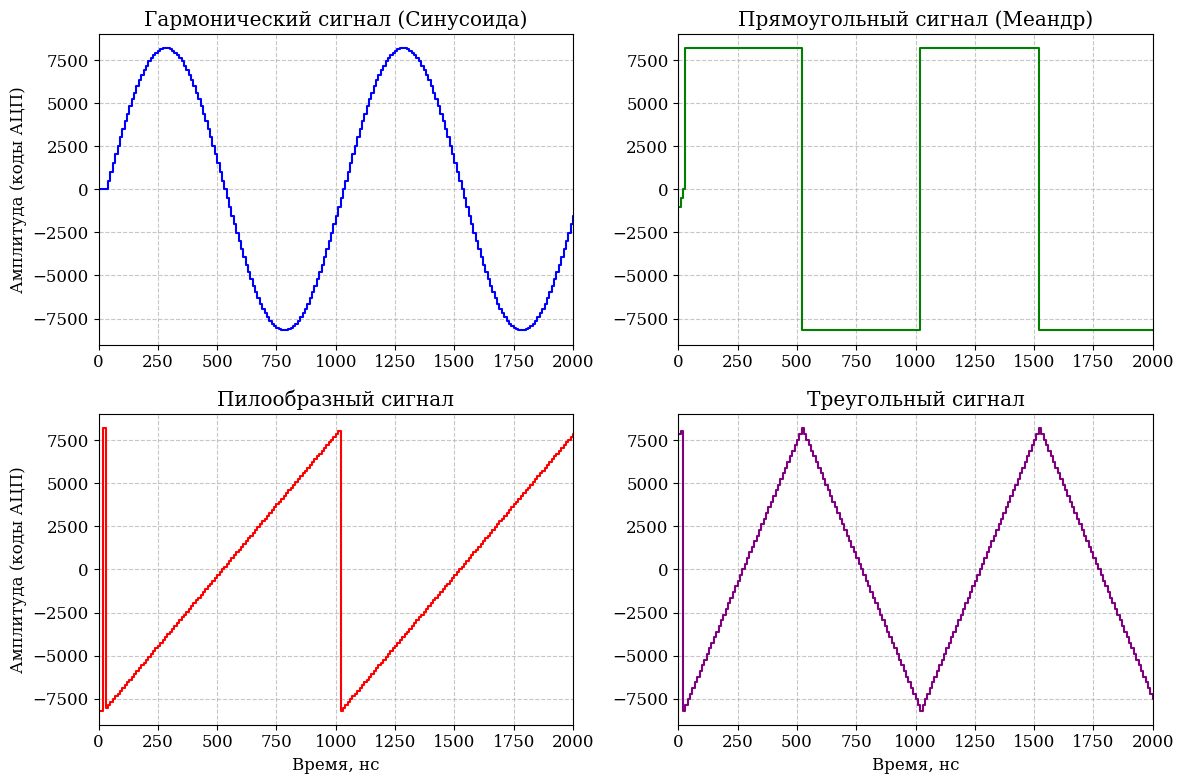
\includegraphics[width=0.9\linewidth]{assets/default_examples.png}
    \caption{Временные диаграммы генерации базовых форм сигналов}
    \label{fig:sim_base_waves}
\end{figure}

В первую очередь оценивалась математическая корректность работы фазового аккумулятора и блока генерации форм. На рисунке \ref{fig:sim_base_waves} представлены результаты симуляции базовых режимов работы устройства.

Анализ полученных осциллограмм подтверждает отсутствие фазового разрыва и выбросов в моменты переполнения фазового аккумулятора. Мультиплексор форм сигналов безошибочно переключает поток данных, а логические операции над битами фазы обеспечивают строго линейное нарастание и спад для пилообразного и треугольного сигналов.

\begin{figure}[htpb]
    \centering
    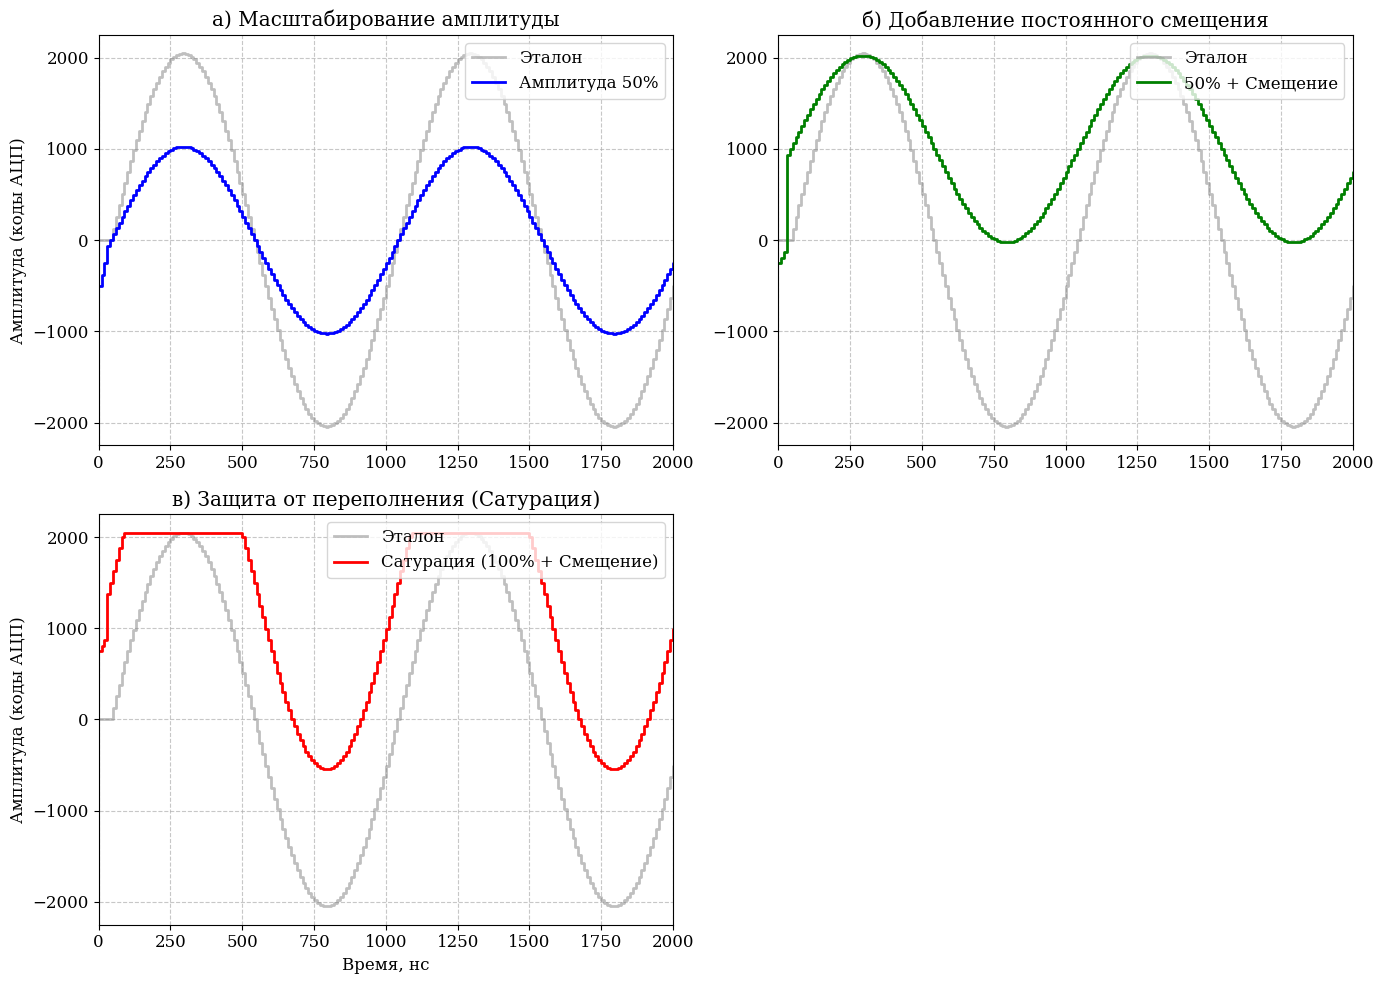
\includegraphics[width=0.9\linewidth]{assets/feature_examples.png}
    \caption{Верификация алгоритмов настройки амлпитуды, смещения и защиты от переполнения}
    \label{fig:sim_dsp_features}
\end{figure}

Вторым этапом верификации стала проверка работоспособности конвейерного блока цифровой обработки (DSP), отвечающего за применение пользовательских настроек к сгенерированному отсчету. Для комплексного тестирования была проведена серия симуляций с различными управляющими векторами, результаты которых объединены на рисунке \ref{fig:sim_dsp_features}.

На фрагментах \textit{а} и \textit{б} продемонстрирована корректная отработка конвейерного умножителя и сумматора: амплитуда сигнала линейно масштабируется заданным коэффициентом, а добавление константы смещения сдвигает график по вертикали без искажения формы исходной волны. 

Особое внимание следует уделить фрагменту \textit{в}, который иллюстрирует работу алгоритма сатурации. При попытке программного задания параметров амплитуды и смещения, сумма которых превышает разрядную сетку выходного интерфейса, цифровой код ограничивается (обрезается) по максимально допустимому значению. Реализация данного защитного механизма является критически важной, так как она надежно предотвращает целочисленное переполнение (wrap-around), которое на практике привело бы к резкой аппаратной инверсии фазы сигнала на выходе цифро-аналогового преобразователя.

Таким образом, результаты поведенческого моделирования полностью подтверждают логическую работоспособность всех спроектированных узлов генератора. Разработанная RTL-модель признана корректной и готовой к этапам логического синтеза, трассировки и загрузки в конфигурационную память отладочной платы ПЛИС.


\subsection{Логический синтез и оценка аппаратных затрат}
После завершения функционального моделирования был выполнен этап логического синтеза и трассировки разработанного RTL-описания. В качестве САПР использовалась среда Xilinx Vivado. Целевой платформой выступала ПЛИС Artix-7.

Для оценки эффективности разработанной архитектуры был произведен анализ потребляемых ресурсов кристалла. Сводные результаты имплементации представлены в таблице \ref{tab:utilization}.

% \begin{figure}[htpb]
%     \centering
%     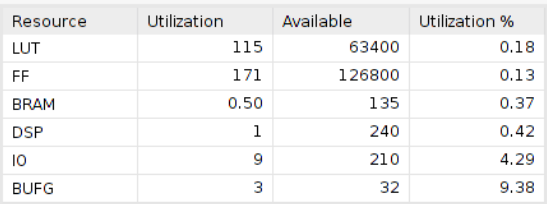
\includegraphics[width=1.0\linewidth]{assets/utilization.png}
%     \caption{Отчет потребления ресурсов ПЛИС, собранный САПР Xilinx Vivado}
%     \label{fig:utilization}
% \end{figure}

\begin{table}[htpb]
    \centering
    \caption{Утилизация ресурсов ПЛИС Artix-7}
    \label{tab:utilization}
    \resizebox{\textwidth}{!}{
    \begin{tabular}{|l|c|c|c|}
        \hline
        \textbf{Тип ресурса} & \textbf{Использовано} & \textbf{Доступно} & \textbf{Использование (\%)} \\
        \hline
        LUT & 115 & 63400 & 0.18 \\
        \hline
        Триггеры & 171 & 126800 & 0.13 \\
        \hline
        Блочная память & 0.5 & 135 & 0.37 \\
        \hline
        Умножители & 1 & 240 & 0.42 \\
        \hline
        Линии ввода-вывода & 9 & 210 & 4.29 \\
        \hline
        Глобальные буферы (BUFG) & 3 & 32 & 9.38 \\
        \hline
    \end{tabular}
    }
\end{table}

Как видно из таблицы \ref{tab:utilization}, устройство отличается низким потреблением ресурсов ПЛИС. Использование 115 LUT и 171 триггера подтверждает эффективность выбранной архитектуры прямого цифрового синтеза.

В проекте задействован один умножитель DSP48E1, который, как было сказано ранее, выполняет функцию масштабирования амплитуды и смещения. Потребление 0.5 примитива BRAM полностью соответствует рассчитаному объему, необходимому для хранения четвертьволновой таблицы значений синуса. В целом, разработанный ГССФ занимает менее $0.5\%$ вычислительных ресурсов кристалла, что оставляет запас для интеграции генератора в качестве IP-ядра в состав более сложных систем на кристалле или для создания многоканальных версий устройства.

По данным отчета об энергопотреблении, представленном в таблице \ref{tab:power}, расчетная статическая и динамическая рассеиваемая мощность на кристалле составляет всего $0.111$ Вт при температуре перехода $25.5\ ^\circ\text{C}$. Столь низкое энергопотребление позволяет использовать устройство в портативной измерительной аппаратуре без применения активных систем охлаждения.

\begin{table}[htpb]
    \centering
    \caption{Результаты анализа энергопотребления в среде Xilinx Vivado}
    \label{tab:power}
    \resizebox{0.7\linewidth}{!}{
    \begin{tabular}{|l|c|}
        \hline
        Total On-Chip Power: & \textbf{0.111 W} \\
        \hline
        Junction Temperature: & \textbf{25.5 °C} \\
        \hline
        Thermal Margin: & 59.5 °C (12.9 W) \\
        \hline
        Effective $\vartheta$JA: & 4.6 °C/W \\
        \hline
        Power supplied to off-chip devices: & 0 W \\
        \hline
    \end{tabular}
    }
\end{table}

\subsubsection{Временной анализ}

Критически важным этапом проектирования синхронных цифровых систем является удовлетворение временных ограничений. Временной анализ проводился для системной тактовой частоты $f_{clk} = 100$ МГц и частоты интерфейса SPI 25 МГц. Результаты временного анализа представлены в таблице \ref{tab:timing}.

\begin{table}[htpb]
    \centering
    \caption{Результаты временного анализа в среде Xilinx Vivado}
    \label{tab:timing}
    \resizebox{0.5\linewidth}{!}{
    \begin{tabular}{|l|c|}
        \hline
        Worst Negative Slack (WNS) & 5.312 ns \\
        \hline
        Total Negative Slack (TNS) & 0 ns  \\
        \hline
        Number of Failing Endpoints & 0 \\
        \hline
        Total Number of Endpoints & 164 \\
        \hline
    \end{tabular}
    }
\end{table}

Отчет статического временного анализатора (Static Timing Analysis, STA) среды Vivado подтвердил полное отсутствие временных нарушений. Количество сбойных путей равно нулю, а суммарный отрицательный запас времени составляет $0$ нс.

Значение наихудшего запаса времени по установке (Worst Negative Slack, WNS) составило $5.312$ нс. Данный результат свидетельствует о том, что максимальная задержка распространения сигнала в комбинационных путях конвейера составляет менее $4.7$ нс. 

Столь значительный временной запас по WNS, составляющий более $50\%$ от периода тактового сигнала, доказывает высокую эффективность введенной конвейеризации и использования выравнивающих регистров. При необходимости, текущая архитектура позволяет без внесения изменений в RTL-код увеличить тактовую частоту генератора почти вдвое до $\approx 180-200$ МГц, что пропорционально расширит спектр генерируемых частот и повысит разрешение по времени.

\section{Экспериментальные исследования и испытания ГССФ}

Заключительным этапом разработки является практическая проверка работоспособности спроектированного устройства на реальном оборудовании. 

Основной целью данных исследований является подтверждение соответствий характеристик готового устройства теоретическим расчетам и результатам функционального моделирования. В ходе испытаний оценивается точность установки частоты, качесвто формирования различных типов сигналов и стабильность работы ЦАП.

\subsection{Описание экспериментальной установки и оборудования}

Для проведения испытаний системы и верификации примененных алгоритмов была собрана экспериментальная установка. В состав тестового стенда входят следующие компоненты:

\begin{enumerate}
    \item Отладочная плата на базе ПЛИС Artix-7. Эта платформа выступает в качестве вычислительного ядра системы, реализуя описанную ранее архитектуру DDS и контроллеры интерфейсов.
    \item Модуль цифро-аналогового преобразователя Pmod DA2. Модуль построен на базе микросхемы DAC121S101 и обеспечивает 12-битную точность преобразования. Соединение с ПЛИС выполнено через стандартный разъем Pmod, обеспечивающий минимальные наводке при передаче высокочастотных сигналов интерфейса SPI. Опорное напряжение ЦАП составляет $\approx 3.3$ В \cite{dac121s101}, что определяет динамический диапазон выходного сигнала.
    \item Цифровой осциллограф КОМ3 С7-304. Данный прибор использовался для визуализации формы выходного сигнала и измерения его характеристик. Основные параметры осциллографа \cite{oscilloscope}:
    \begin{itemize}
        \item полоса пропускания: до 1000 МГц, что позволяет наблюдать гармоники и переходные процессы без существенных искажений;
        \item частота дискретизации: до 5 ГГц;
        \item наличие функции автоматических измерений и спектрального анализа на основе БПФ.
    \end{itemize}
    \item Персональный компьютер с установленной средой проектирования Xilinx Vivado. ПК использовался для загрузки конфигурационного файла в ПЛИС и оперативного управления параметрами генерации через интерактивную панель Virtual Input/Output.
\end{enumerate}

\begin{figure}[htpb]
    \centering
    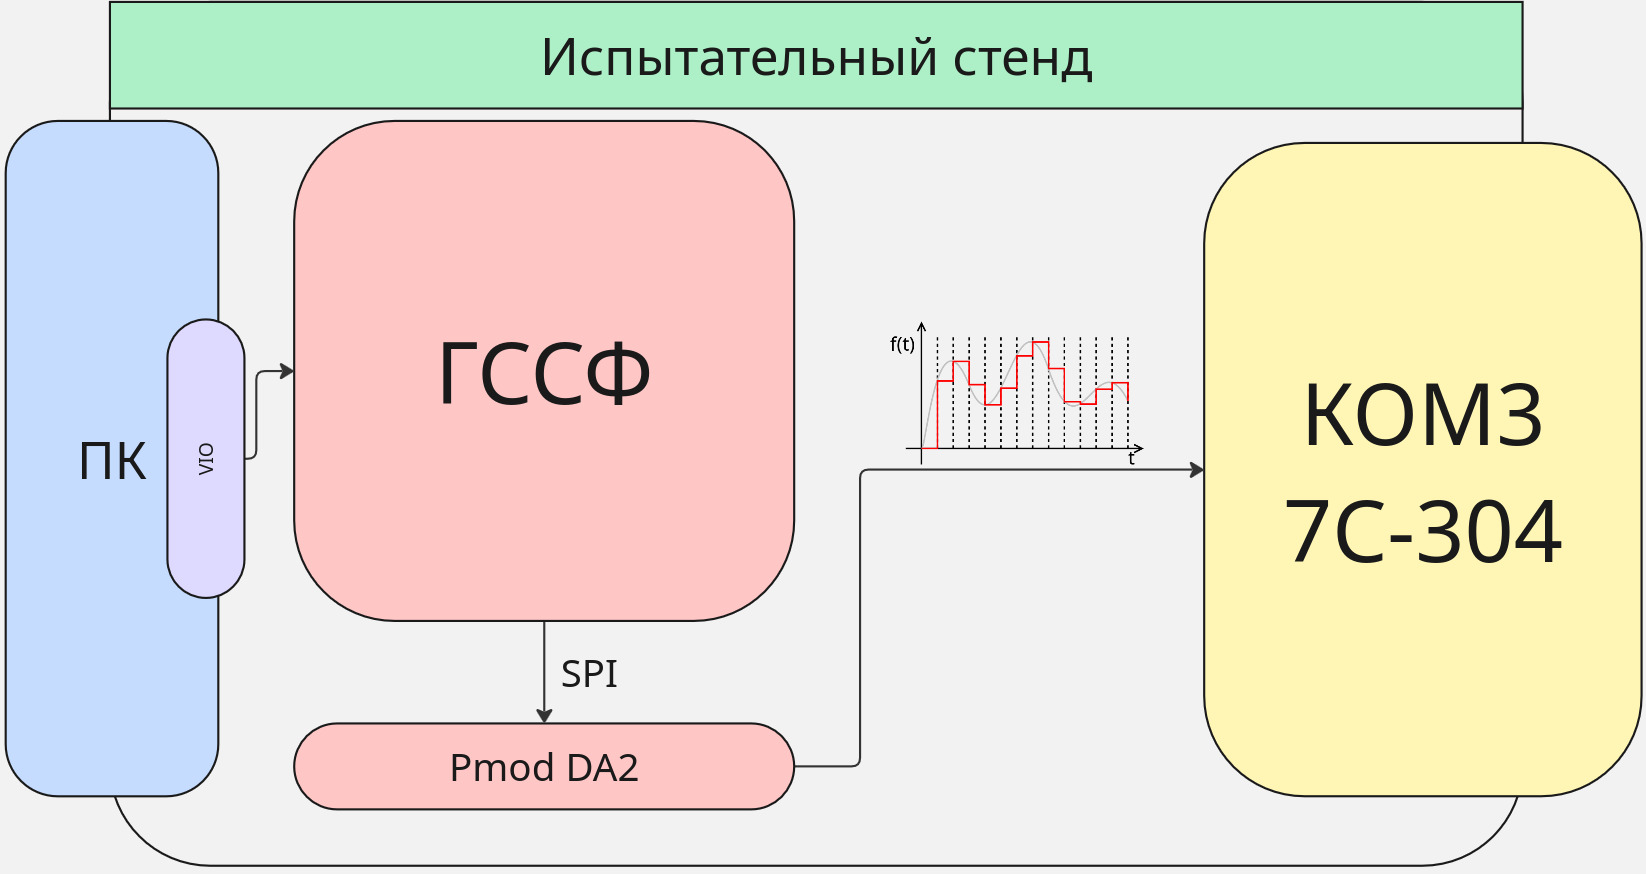
\includegraphics[width=1\linewidth]{assets/struct_scheme_test_stand.jpg}
    \caption{Структурная схема испытательного стенда}
    \label{fig:struct_setup}
\end{figure}

Общая схема информационных потоков в установке представлена на рисунке \ref{fig:struct_setup}. Управляющие команды поступают с ПК через интерфейс JTAG в ПЛИС. Вычислительное ядро формирует цифровые отсчеты, которые по протоколу SPI передаются на модуль ЦАП. Аналоговый сигнал с выхода ЦАП подается на вход осциллографа через коаксиальный кабель с согласованным импедансом 50 Ом для минимизации отражений сигнала.

\subsection{Методика программирования и настройки ПЛИС}

Процесс подготовки устройства к работе включал этапы логического синтеза, трассировки и генерации битового потока в среде Xilinx Vivado. Загрузка конфигурации в ПЛИС Artix-7 осуществлялась через аппаратный менеджер (Hardware Manager, HW) по интерфейсу JTAG.

Процесс логического синтеза преобразует исходное RTL-описание в список цифровых блоков и соединений, из набора примитивов, предоставленной программе, библиотеки. Полученный список связей называется нетлист. После логического синтеза начинается этап трассировки. Программа выбирает из доступных на кристалле элементов, необходимые для реализации нетлиста, оптимизирует схему, затем генерируется результирующий битовый поток, готовый для загрузки в ПЛИС.

\begin{figure}[htpb]
    \centering
    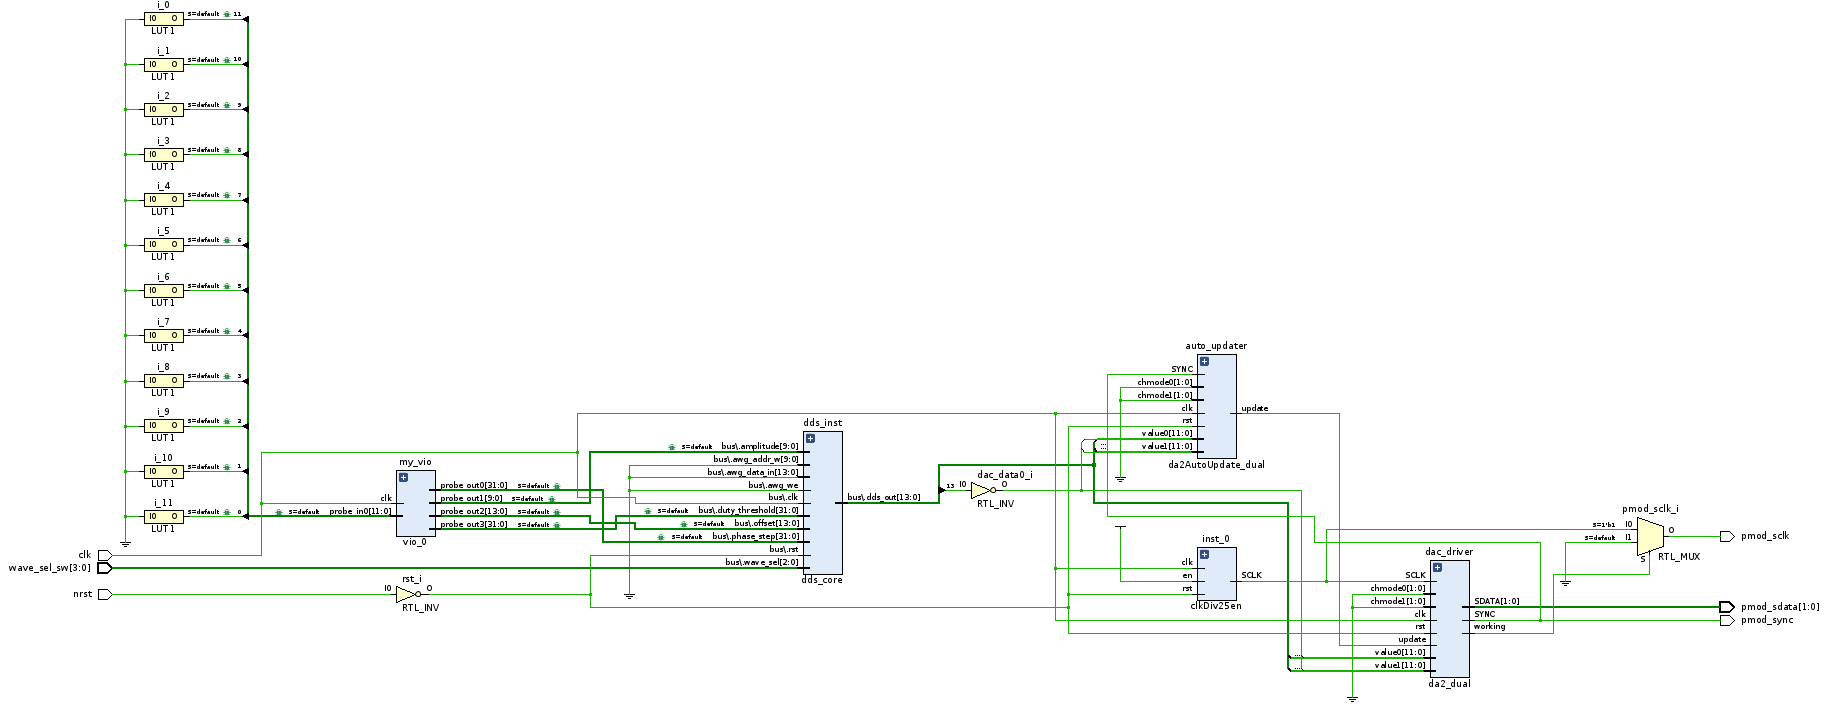
\includegraphics[width=1\linewidth]{assets/Screenshot from 2026-04-25 12-48-00.png}
    \caption{Схема электрическая структурная (Elaborated Design) верхнего уровня}
    \label{fig:rtl_top}
\end{figure}

\begin{figure}[htpb]
    \centering
    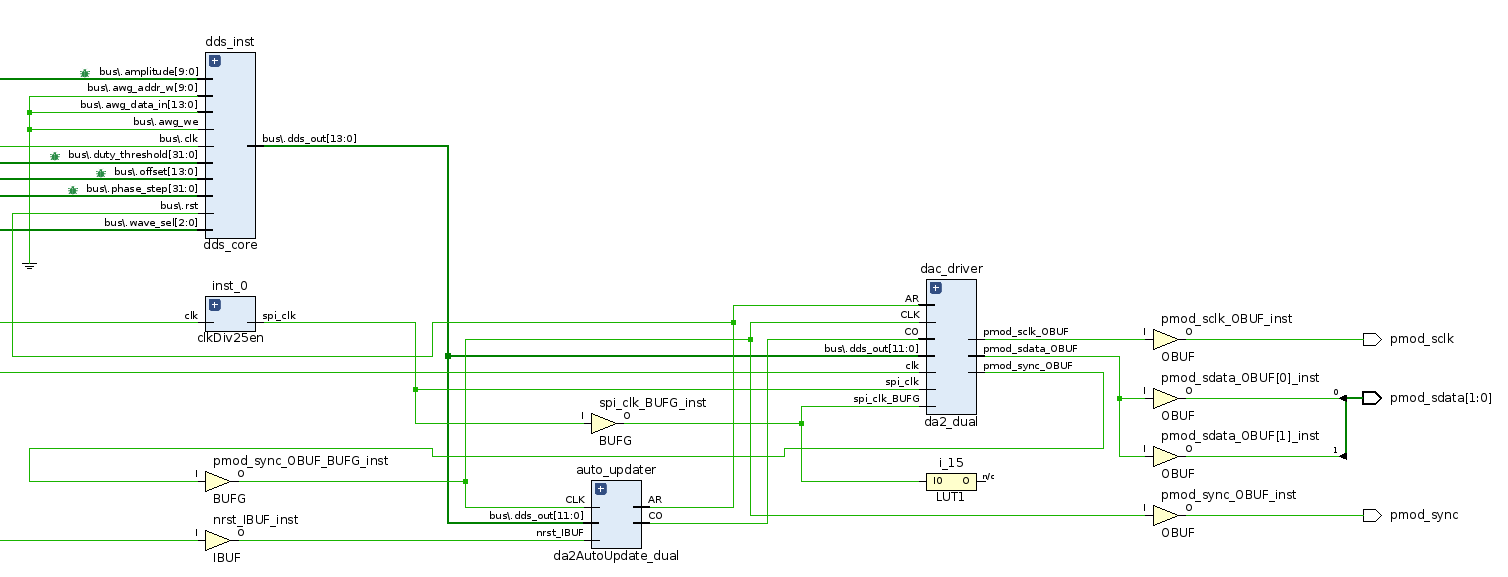
\includegraphics[width=1\linewidth]{assets/Screenshot from 2026-04-25 12-52-48.png}
    \caption{Трассировка тактовых цепей и выходных каскадов интерфейса SPI}
    \label{fig:rtl_spi}
\end{figure}

Анализ схем подтверждает корректную интеграцию всех ключевых подсистем: вычислительного ядра \texttt{dds\_core}, модуля виртуальных вводов-выводов \texttt{my\_vio} и контроллера интерфейса SPI \texttt{dac\_driver}. Особое внимание на этапе синтеза было уделено маршрутизации тактовых сигналов: для тактирования SPI-интерфейса используются специализированные глобальные буферы (\texttt{BUFG}), а для высокочастотных сигналов — выходные буферы (\texttt{OBUF}).

После логического синтеза начинается этап трассировки и привязки логических портов проекта к физическим аппаратным выводам микросхемы (I/O Planning).

\begin{figure}[htpb]
    \centering
    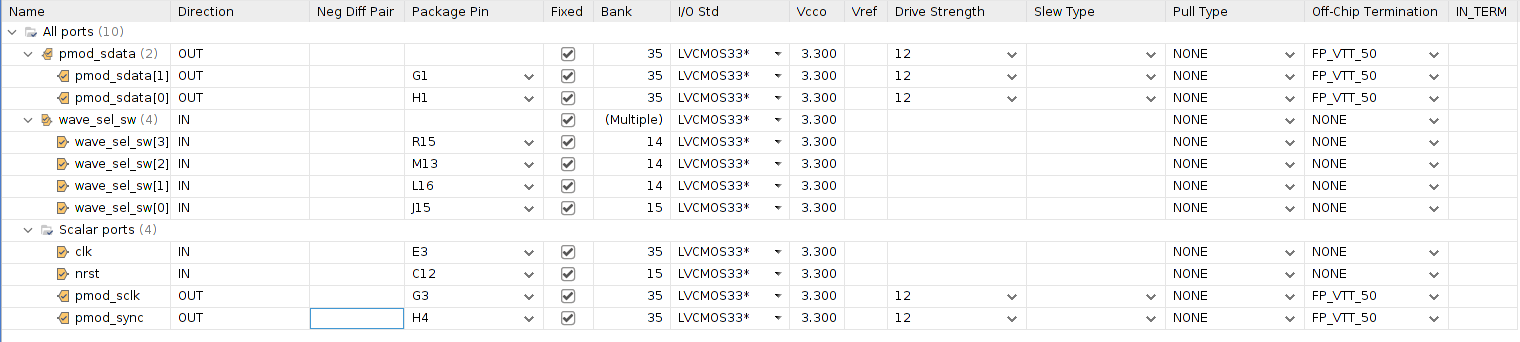
\includegraphics[width=1\linewidth]{assets/Screenshot from 2026-04-25 12-54-06.png}
    \caption{Назначение выводов (Pin Planner) и стандартов ввода-вывода}
    \label{fig:pin_planner}
\end{figure}

Как видно из рисунка \ref{fig:pin_planner}, для обеспечения совместимости с модулем Pmod DA2 всем выходным сигналам интерфейса SPI был жестко назначен стандарт ввода-вывода LVCMOS с уровнем напряжения 3.3 В. Назначение конкретных выводов корпуса производилось в строгом соответствии с принципиальной схемой используемой отладочной платы.

Сгенерированный результирующий битовый поток (Bitstream) загружался в целевую ПЛИС \texttt{xc7a100t\_0} с использованием Vivado Hardware Manager.

\begin{figure}[htpb]
    \centering
    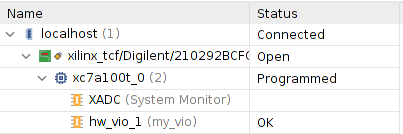
\includegraphics[width=0.8\linewidth]{assets/Screenshot from 2026-04-25 13-46-50.png}
    \caption{Состояние аппаратного менеджера после загрузки конфигурации}
    \label{fig:hw_manager}
\end{figure}

Успешная конфигурация кристалла подтверждается статусом \textit{Programmed} на рисунке \ref{fig:hw_manager}. Диспетчер устройств также зафиксировал активное состояние интегрированного логического анализатора и панели управления \texttt{hw\_vio\_1} (статус \textit{OK}), что обеспечило возможность проведения дальнейших интерактивных испытаний ГССФ.

Для управления параметрами генератора в реальном времени, без необходимости перекомпиляции проекта, в состав прошивки интегрирован отладочный модуль VIO. На стороне хост-компьютера была создана интерактивная панель управления со следующими элементами:
\begin{itemize}
    \item \texttt{wave\_sel [2:0]} - переключатель формы сигнала;
    \item \texttt{phase\_step [31:0]} - установка значения инкремента фазы для изменения частоты;
    \item \texttt{amplitude [11:0]} - управление коэффициентом усиления в блоке DSP;
    \item \texttt{offset [11:0]} - задание смещения постоянной составляющей;
    \item \texttt{duty\_threshold [31:0]} - настройка скважности прямоугольного сигнала.
\end{itemize}

Данный подход позволил проводить испытания в динамическом режиме, плавно изменяя частоту выходного сигнала и наблюдая за реакцией аппаратной части и внешного ЦАП.

\subsection{Результаты генерации стандартных форм сигналов}

В данном разделе представлены результаты натурных испытаний ГССФ в режимах синтеза стандартных форм колебаний. Переключение режимов осуществлялось путем изменения конфигурационного вектора \texttt{wave\_sel} через интерфейс VIO.

В качестве опорной частоты для первой серии измерений была выбрана тестовая частота $f_{test} = 1$ кГц. Для ее генерации, согласно формуле \eqref{eq:1}, в регистр \texttt{phase\_step} было записано соответствующее целочисленное значение:
\[
    \Delta \Theta = \frac{f_{test} 2^M}{f_{clk}}
\]
\[ \Delta \Theta = \frac{1 \text{кГц} \cdot 2^{32}}{100 \text{МГц}} \approx 42950 \]

\subsubsection{Синтез гармонических сигналов}
На рисунке \ref{fig:osc_sine} представлена осциллограмма синусоидального сигнала, синтезированного с использованием алгоритма QWS и внутренней памяти BRAM ПЛИС.

\begin{figure}[htpb]
    \centering
    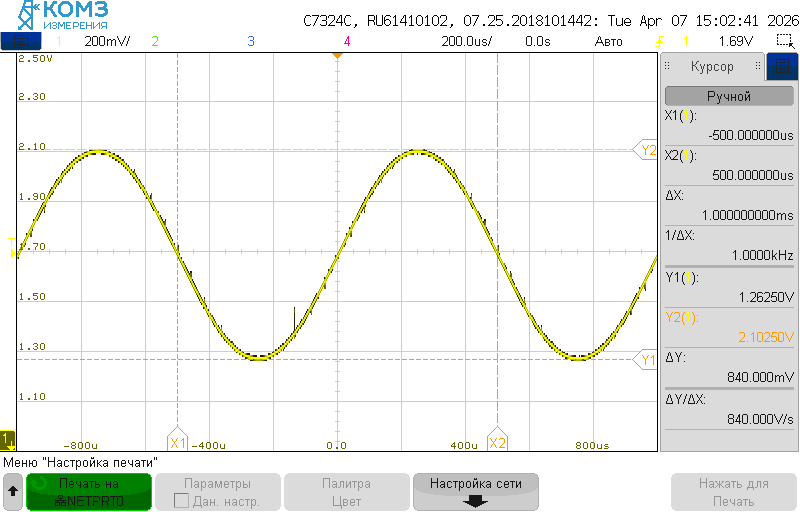
\includegraphics[width=0.8\linewidth]{assets/scope_0.png} % Замени на свое фото
    \caption{Осциллограмма синусоидального сигнала на выходе ЦАП частотой 1 кГц}
    \label{fig:osc_sine}
\end{figure}

Как видно из представленной осциллограммы, генератор успешно формирует периодический гармонический сигнал c ограниченной амплитудой и постоянным смещением. Встроенная функция измерений осциллографа зафиксировала частоту сигнала, которая с высокой точностью совпадает с расчетным значением, заданным в управляющем интерфейсе. Это подтверждает полную математическую корректность работы 32-разрядного фазового аккумулятора.

\begin{figure}[htpb]
    \centering
    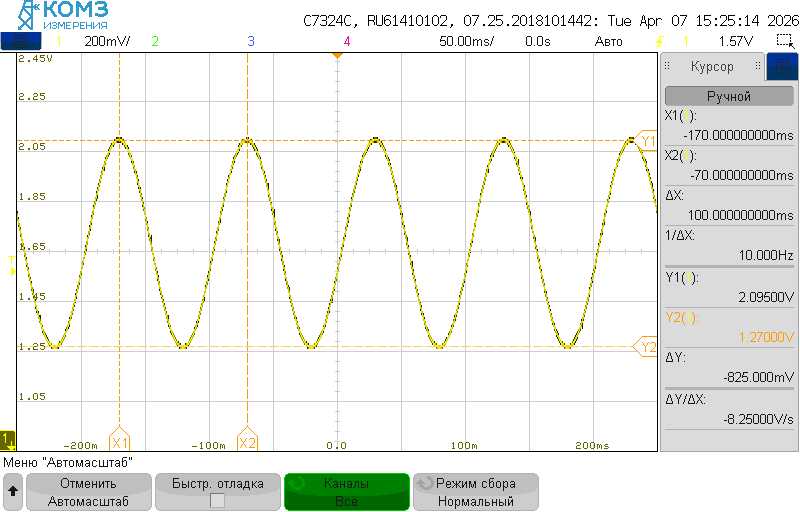
\includegraphics[width=0.8\linewidth]{assets/sin-10Hz.png} % Замени на свое фото
    \caption{Осциллограмма синусоидального сигнала на выходе ЦАП частотой 10 Гц}
    \label{fig:osc_sine_10Hz}
\end{figure}

На рисунке \ref{fig:osc_sine_10Hz} представлена осциллограмма синусоиды сгенерированной с частотой 10 Гц, что демонстрирует возможность генератора синтезировать сигналы с большим периодом колебаний.

Для сигналов с такой частотой, ступеньки после ЦАП незаметны, поскольку наблюдается случай передискретизации (oversampling). Опорная частота ПЛИС $f_{clk} = 100$ МГц. При генерации сигнала 1 кГц, за один период синусоиды на ЦАП попадает $N=\frac{100\cdot 10^6}{1\cdot 10^3}$ точек. Ступеньки длятся около 10 наносекунд, при развертке осциллографа 200 мкс/дел, луч физически не успевает отрисовать ступеньки, поэтому они сливаются в гладкую линию.

\subsubsection{Синтез импульсных и линейно-изменяющихся сигналов}

Помимо гармонических колебаний, разработанный ГССФ поддерживает аппаратную генерацию стандартных измерительных сигналов: пилообразного, треугольного и прямоугольного. В отличие от синусоиды, данные формы формируются без использования блочной памяти (BRAM), исключительно за счет комбинационных логических операций над старшими битами усеченного кода фазы.

На рисунках \ref{fig:osc_saw} и \ref{fig:osc_tri} показаны осциллограммы пилообразного и треугольного сигналов.

\begin{figure}[htpb]
    \centering
    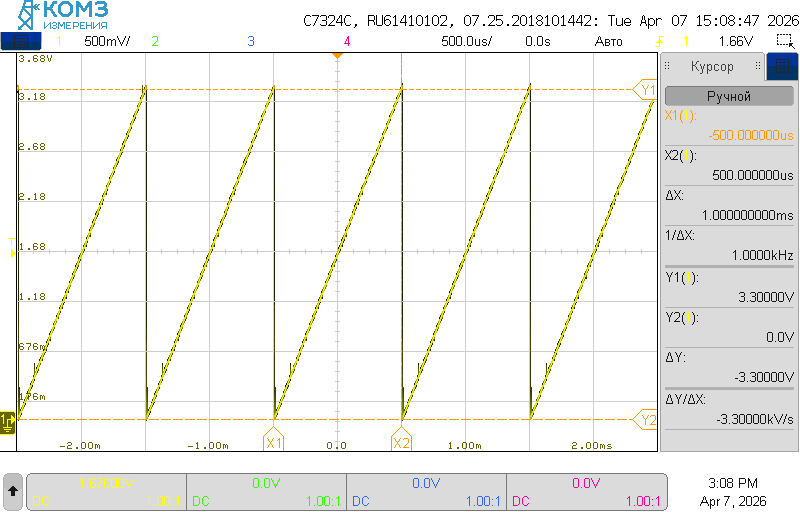
\includegraphics[width=0.8\linewidth]{assets/saw.png} % Замени на свое фото пилы
    \caption{Осциллограмма пилообразного сигнала}
    \label{fig:osc_saw}
\end{figure}

\begin{figure}[htpb]
    \centering
    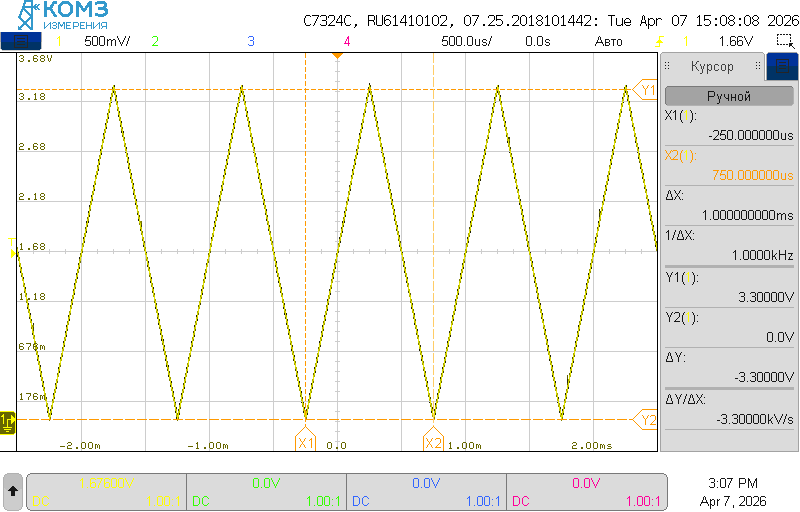
\includegraphics[width=0.8\linewidth]{assets/triangle.png} % Замени на свое фото треугольника
    \caption{Осциллограмма треугольного сигнала}
    \label{fig:osc_tri}
\end{figure}

Анализ полученных осциллограмм подтверждает высокую линейность участков нарастания и спада напряжения. Для пилообразного сигнала характерен мгновенный спад амплитуды от максимального значения к нулю, что физически соответствует моменту аппаратного переполнения 32-разрядного фазового аккумулятора. 

При детальном исследовании данного переходного процесса (рисунок \ref{fig:osc_saw_fall}) с помощью курсорных измерений было зафиксировано, что время спада напряжения составляет $\approx 2.56$ мкс.

\begin{figure}[htpb]
    \centering
    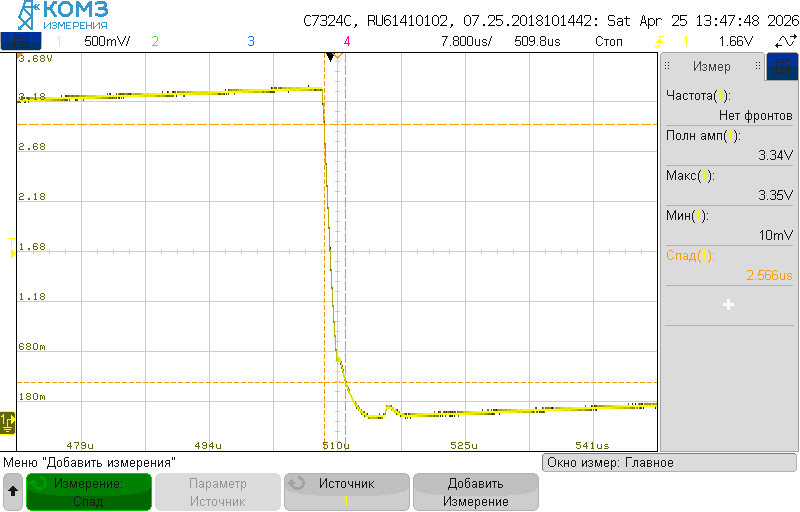
\includegraphics[width=0.8\linewidth]{assets/osc_saw_fall.png}
    \caption{Измерение времени спада пилообразного сигнала}
    \label{fig:osc_saw_fall}
\end{figure}

Наличие данного временного интервала обусловлено не задержками в цифровом вычислительном ядре, где сброс аккумулятора фазы происходит за один такт системной частоты 100 МГц, а динамическими характеристиками микросхемы DAC121S101 \cite{dac121s101}. Конечная скорость нарастания и спада выходного напряжения (Slew Rate) и время установления (Settling Time) ЦАП определяют итоговую форму фронтов. При частоте сигнала 1 кГц данный интервал занимает менее $0.3\%$ от периода, что обеспечивает высокую визуальную линейность.

Для прямоугольного сигнала (меандра) ключевым тестируемым параметром являлась возможность аппаратной регулировки скважности в реальном времени. Формирование прямоугольного сигнала осуществляется с помощью цифрового компаратора, порог срабатывания которого задается регистром \texttt{duty\_threshold}.

\begin{figure}[htpb]
    \centering
    \begin{minipage}{0.48\textwidth}
        \centering
        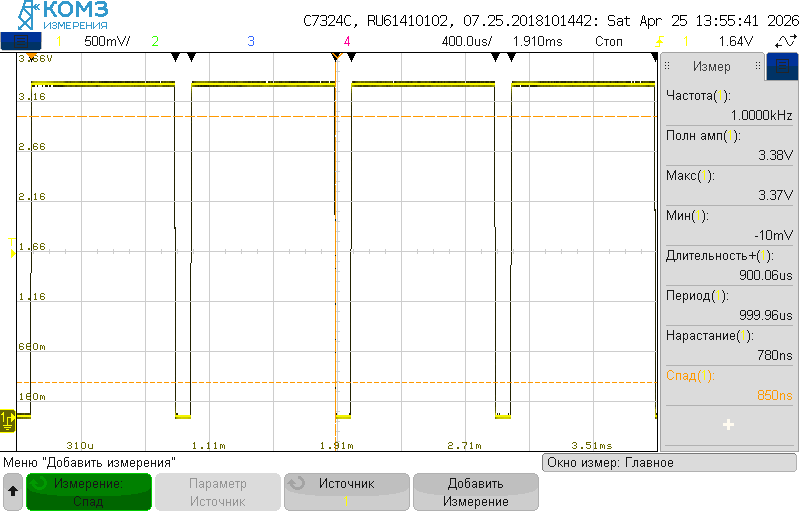
\includegraphics[width=1\linewidth]{assets/square-10-1kHz.png} % Фото 10%
        \caption{Прямоугольный сигнал, скважность 1.1}
        \label{fig:sq_10}
    \end{minipage}\hfill
    \begin{minipage}{0.48\textwidth}
        \centering
        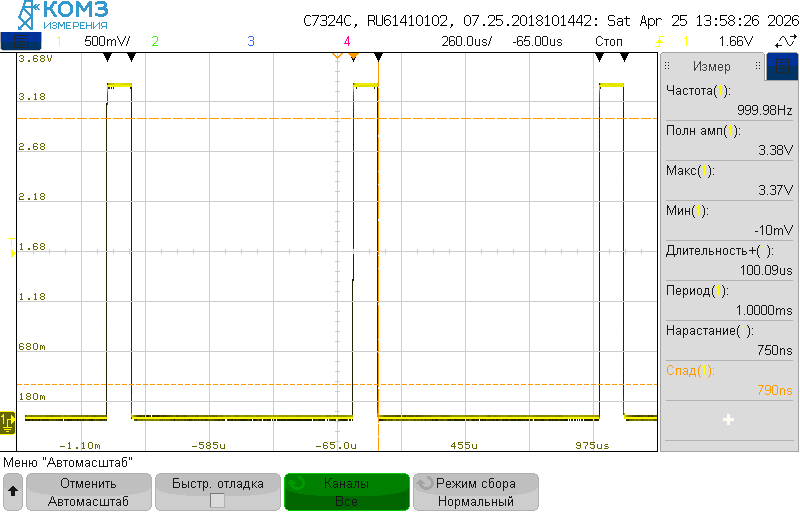
\includegraphics[width=1\linewidth]{assets/square-90-1kHz.png} % Фото 90%
        \caption{Прямоугольный сигнал, скважность 10}
        \label{fig:sq_90}
    \end{minipage}
\end{figure}

На рисунках \ref{fig:sq_10} и \ref{fig:sq_90} представлены осциллограммы прямоугольных импульсов со скважностью 1.1 и 10 соответственно. Как видно из осциллограмм, изменение управляющего параметра в интерактивной панели VIO вызывает строго пропорциональное изменение ширины импульса (100 мкс и 900 мкс) при неизменном фундаментальном периоде равном 1 мс. Это подтверждает корректность математической модели цифрового ШИМ-модулятора.

\subsection{Исследование режима генерации сигналов произвольной формы}

Главным отличием разработанного ГССФ от простейших DDS-синтезаторов является поддержка режима генерации сигналов произвольной формы. Для реализации данного функционала в архитектуру устройства интегрирована двухпортовая блочная память ПЛИС.

Загрузка пользовательского массива отсчетов осуществляется в асинхронном режиме. При переключении вектора \texttt{wave\_sel} в режим AWG, вычислительное ядро DDS начинает использовать старшие биты фазового аккумулятора в качестве указателя для непрерывного циклического чтения отсчетов из памяти.

В качестве тестового сигнала произвольной формы был выбран амплитудно-модулированный радиоимпульс. Математически данный сигнал описывается как произведение высокочастотного несущего колебания и низкочастотной огибающей:

\begin{equation}
    y(t) = \sin(2\pi f_c t) \cdot \sin(\pi f_m t)
\end{equation}

Визуально огибающая такого сигнала имеет характерную веретенообразную форму. Выбор данного паттерна обусловлен тем, что он наглядно демонстрирует способность генератора аппаратно воспроизводить сложные радиотехнические сигналы с динамически изменяющейся амплитудой, применяемые в системах телекоммуникации.

Для проведения эксперимента массив из 4096 дискретных отсчетов был предварительно рассчитан программным путем, отмасштабирован в 12-битный беззнаковый диапазон ЦАП и загружен в память ПЛИС.

\begin{figure}[htpb]
    \centering
    % \includegraphics[width=0.8\linewidth]{assets/fish_signal.png}
    \caption{Осциллограмма сигнала произвольной формы}
    \label{fig:osc_awg_fish}
\end{figure}

Анализ осциллограммы (рисунок \ref{fig:osc_awg_fish}) подтверждает возможность аппаратной реконструкции сложного сигнала. Микросхема ЦАП DAC121S101 корректно отрабатывает плавные изменения амплитуды без искажений огибающей, что доказывает полную работоспособность разработанного интерфейса прямого доступа к памяти и готовность генератора к воспроизведению любых пользовательских паттернов.

\subsection{Анализ точности, спектральной чистоты и аппаратных ограничений}

Для глубокой оценки качества формируемых гармонических колебаний был проведен спектральный анализ выходного напряжения с использованием функции быстрого преобразования Фурье, встроенной в осциллограф С7-304.

\begin{figure}[htpb]
    \centering
    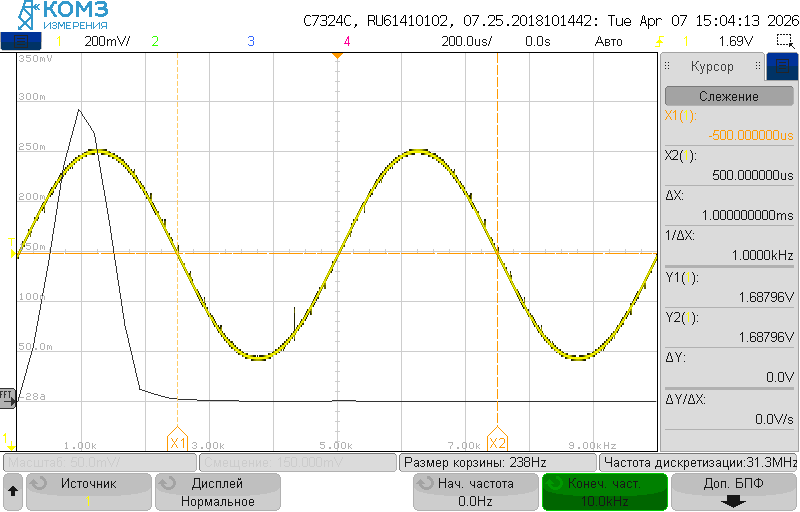
\includegraphics[width=0.8\linewidth]{assets/bpf-sin-1k.png}
    \caption{Спектрограмма синусоидального сигнала частотой 1 кГц}
    \label{fig:fft_1k}
\end{figure}

Анализ спектрограммы на рисунке \ref{fig:fft_1k} демонстрирует ярко выраженный узкий основной лепесток на частоте 1 кГц. Отсутствие значимых высших гармоник и побочных спектральных составляющих в прилегающей полосе подтверждает высокий динамический диапазон. Высокий коэффициент передискретизации и 12-битное разрешение ЦАП обеспечивают крайне низкий уровень шума квантования.

Вместе с тем, в ходе исследований была выявлена физическая граница применимости генератора, обусловленная пропускной способностью интерфейса SPI. При тактовой частоте SPI $f_{SPI} = 25$ МГц и длине кадра 16 бит, максимальная частота обновления ЦАП составляет $f_s \approx 1.56$ MSPS.

При попытке генерации частот свыше 100 кГц, когда на один период приходится менее 15 отсчетов на экране осциллографа наблюдается выраженная деградация формы сигнала. Поскольку количество отсчетов на период не является целым числом, фаза выборки постоянно смещается, что приводит к эффекту биений и визуальному «раздвоению» линий на экране. Данный артефакт является классическим проявлением зеркальных частот экстраполятора нулевого порядка в условиях отсутствия аналогового ФНЧ. Это доказывает, что для синтеза мегагерцовых частот архитектура требует применения параллельных ЦАП.

\subsection{Динамическое управление параметрами синтеза и свойство непрерывности фазы}

Для демонстрации данного свойства и тестирования отзывчивости системы управления был проведен эксперимент по генерации частотно-манипулированных сигналов (FSK), имитирующих воспроизведение музыкального звукоряда. Через отладочный интерфейс в регистр генератора последовательно загружались коды инкремента фазы, соответствующие стандартным нотам равномерно темперированного строя.

В ходе натурного прослушивания и анализа переходных процессов на осциллографе было подтверждено отсутствие паразитных амплитудных скачков в моменты переключения частот. Данный тест доказывает абсолютную непрерывность фазы выходного сигнала. Подобная гибкость управления позволяет использовать разработанное ядро ГССФ не только в качестве лабораторного прибора, но и как базовый блок для цифровых модуляторов в системах телекоммуникации.

\section*{Заключение}
\addcontentsline{toc}{section}{Заключение}

В ходе выполнения выпускной квалификационной работы была решена актуальная научно-техническая задача - разработан и аппаратно-программным способом реализован прецизионный генератор сигналов специальной формы на базе программируемой логической интегральной схемы  семейства Artix-7. Поставленная цель исследования достигнута, а все заявленные задачи выполнены в полном объеме.

В процессе работы был проведен глубокий сравнительный анализ методов генерации сигналов. Теоретически обосновано и практически доказано преимущество метода прямого цифрового синтеза в сочетании с ресурсами встроенной блочной памяти ПЛИС для задач, требующих мгновенной перестройки частоты и формирования сигналов произвольной формы \cite{shunli, analog-dds}.

На языке аппаратного описания SystemVerilog спроектировано строго синхронное конвейерное вычислительное ядро. Применение алгоритма четвертьволновой симметрии позволило оптимизировать использование ресурсов памяти кристалла, а интеграция аппаратных макроблоков DSP48E1 \cite{dsp48e1} обеспечила высокоскоростное масштабирование амплитуды и надежную аппаратную защиту цифрового тракта от целочисленного переполнения. Для взаимодействия с внешним 12-битным цифро-аналоговым преобразователем Pmod DA2 \cite{dac121s101} разработан надежный контроллер протокола SPI, в котором успешно решена проблема пересечения тактовых доменов.

Адекватность и математическая корректность предложенных архитектурных решений подтверждена на всех этапах маршрута проектирования. Функциональное моделирование с использованием методологии псевдослучайного тестирования с ограничениями в объектно-ориентированном тестовом окружении доказало побитовую точность работы вычислительного конвейера во всем диапазоне допустимых значений. Оценка результатов логического синтеза в САПР Xilinx Vivado продемонстрировала высокую ресурсоэффективность архитектуры, было использовано менее 0.5\% базовой логики кристалла, и наличие значительного запаса по временным ограничениям WNS > 5 нс.

Натурные испытания на экспериментальном аппаратном стенде полностью подтвердили результаты расчетов и моделирования. Осциллографические измерения зафиксировали высокую линейность формируемых сигналов, корректную отработку заданных уровней скважности ШИМ-сигнала и успешное воспроизведение сложного амплитудно-модулированного радиоимпульса в режиме прямого доступа к памяти. Спектральный анализ подтвердил высокий динамический диапазон генератора и крайне низкий уровень шума квантования на базовых частотах. Эксперимент с генерацией частотно-манипулированных сигналов практически доказал важнейшее свойство архитектуры DDS - абсолютную непрерывность фазы при динамической перестройке частоты \cite{Vankka}.

Гибкость разработанной модульной архитектуры, низкое энергопотребление и компактность RTL-кода позволяют использовать данный генератор не только как самостоятельный лабораторный инструмент, но и интегрировать его в качестве готового IP-ядра в состав сложных радиотехнических систем на кристалле, комплексов автоматизированного тестирования и современного телекоммуникационного оборудования.

\clearpage
\newpage

\begin{thebibliography}{99}

    \bibitem{Hao_2021}
    Hao, Dawen. (2021). Research on DDS-based Portable Signal Generation Testing Device. Journal of Physics: Conference Series. 1971(1). 012001. doi:10.1088/1742-6596/1971/1/012001.

    \bibitem{shunli}
    Li, Shun. (2024). Design and Implementation of DDS Signal Generator Based on FPGA. Academic Journal of Science and Technology. 9. 145-149.
    
    \bibitem{tierney} 
    Tierney.  A  Digital  frequency  synthesizer  [J]  IEEE  Trans AEV, 1971, 19(1) :48-57 

    \bibitem{analog-dds}
    Cronin B. DDS Devices Generate High-Quality Waveforms Simply, Efficiently, and Flexibly. Analog Dialogue 46-01, 2012.

    \bibitem{Vankka}
    Vankka  J.  Digital  frequency  synthesizer/modulator  for continuous-phase modulations with slow frequency hopping[J]. IEEE transactions on vehicular technology, 1997, 46(4): 933-940. 
    
    \bibitem{arbitrary}
    P. Symons, “DDS arbitrary waveform generation,” in Digital Waveform Generation, Cambridge: Cambridge University Press, 2013, с. 162–227

    \bibitem{spectr}
    Ридико Л. И. DDS: прямой цифровой синтез частоты // Компоненты и технологии. 2001. № 7. с. 50--54.

    \bibitem{cordic}
    Захаров А. В., Хачумов В. М. Алгоритмы CORDIC. Современное состояние и перспективы. М.: Физ-матлит. 2004.

    \bibitem{filipovsky2022}
    Филиповский В. М. Дискретные системы управления. Методические указания к практическим занятиям и лабораторным работам: - СПб.: СПбПУ, 2022. - 61 с.
    
    \bibitem{mcu-shit}
    Kaliappan, S. (2021). Comparative Analysis of FPGA and Microcontroller based Signal Generation for Power Electronics Applications. International Journal of Advanced Research in Electrical, Electronics and Instrumentation Engineering.

    \bibitem{ad9850}
    Analog Devices. CMOS, 125 MHz Complete DDS Synthesizer, AD9850. URL:https://www.analog.com/media/en/technical-documentation/data-sheets/AD9850.pdf (дата обращения 05.03.2026, 20:00)

    \bibitem{dsp48e1}
    7 Series DSP48E1 Slice: User Guide (UG953) / AMD Adaptive Computing. - 2024. URL: https://docs.amd.com/r/en-US/ug953-vivado-7series-libraries/DSP48E1 (дата обращения 18.03.2026, 18:00)

    \bibitem{dac121s101}
    DAC121S101 12-Bit Micro-Power, General Purpose Digital-to-Analog Converter with Rail-to-Rail Output:SNAS303M:datasheet/Texas Instruments. - Rev.Jan.2016.- 18 p. URL:https://www.ti.com/lit/ds/symlink/dac121s101-q1.pdf?ts=1776258599775 (дата обращения 05.03.2026, 21:00)

    \bibitem{oscilloscope}
    Описание типа средства измерений. Осциллографы КОМ3 АльфаТрек серии С7-300. Приложение к свидетельству №73409. - М.: Росстандарт, 2019. - 7 с.
\end{thebibliography}

\newpage
\section*{Приложение А \\ Исходный код верхнего модуля}
\addcontentsline{toc}{section}{Приложение А}
\begin{lstlisting}[language=Verilog, frame=none,caption={RTL-описание верхнего модуля (top.sv)}]
`timescale 1ns/1ps

module dds_dac_top #(
    parameter int AMP_W = 10,
    parameter int PHASE_W = 32,
    parameter int LUT_W = 10,
    parameter int OUT_W = 14,
    parameter int AWG_W = 10
)(
    input  logic       clk,            
    input  logic       nrst,            
    input  logic [2:0] wave_sel_sw,   
    
    output logic [1:0] pmod_sdata,
    output logic       pmod_sync,
    output logic       pmod_sclk
);
    logic rst;
    assign rst = ~nrst;
    logic spi_clk;

    gen_if #(
        .AMP_W(AMP_W),
        .PHASE_W(PHASE_W),
        .LUT_W(LUT_W),
        .OUT_W(OUT_W),
        .AWG_W(AWG_W)
    ) bus_if (
        .clk(clk)
    );
    
    clkDiv25en inst_0 (
        .clk(clk),
        .rst(rst),
        .en('1),
        .SCLK(spi_clk)
    );
    
    wire [31:0] vio_phase_step;
    wire [9:0]  vio_amplitude;
    wire [13:0] vio_offset;
    wire [31:0] vio_duty_threshold;
    wire [11:0] vio_dds_output;
    
    vio_0 my_vio (
        .clk(clk),
        .probe_in0(vio_dds_output),
        .probe_out0(vio_phase_step),
        .probe_out1(vio_amplitude),
        .probe_out2(vio_offset),
        .probe_out3(vio_duty_threshold)
    );
    assign vio_dds_output = '0;

    assign bus_if.rst      	 = rst;
    assign bus_if.wave_sel 	 = wave_sel_sw;
    assign bus_if.phase_step     = vio_phase_step; 
    assign bus_if.amplitude      = vio_amplitude;
    assign bus_if.offset         = vio_offset;
    assign bus_if.duty_threshold = vio_duty_threshold;
    
    assign bus_if.awg_we         = 1'b0;
    assign bus_if.awg_addr_w     = '0;
    assign bus_if.awg_data_in    = '0;

    dds_core #(
        .AMP_W(AMP_W),
        .PHASE_W(PHASE_W),
        .LUT_W(LUT_W),
        .OUT_W(OUT_W),
        .AWG_W(AWG_W)
    ) dds_inst (
        .bus(bus_if.dut)
    );

    logic [11:0] dac_data;
    assign dac_data = {~bus_if.dds_out[OUT_W-1], bus_if.dds_out[OUT_W-2 : 2]};

    wire update_trig;
    wire working_flag;

    da2AutoUpdate_dual auto_updater (
        .clk(clk),
        .rst(rst),
        .SYNC(pmod_sync),
        .update(update_trig),
        .chmode0(2'b00),       
        .chmode1(2'b00),       
        .value0(dac_data),     
        .value1(dac_data)      
    );

    da2_dual dac_driver (
        .clk(clk),
        .rst(rst),
        .SCLK(spi_clk),       
        .SDATA(pmod_sdata),   
        .SYNC(pmod_sync),     
        .working(working_flag),
        .chmode0(2'b00),      
        .chmode1(2'b00),      
        .value0(dac_data),
        .value1(dac_data),
        .update(update_trig)
    );

    assign pmod_sclk = (working_flag) ? spi_clk : 1'b0;

endmodule
\end{lstlisting}

\newpage
\section*{Приложение Б \\ Исходный код вычислительного ядра DDS}
\addcontentsline{toc}{section}{Приложение Б}
\begin{lstlisting}[language=Verilog, frame=none,caption={RTL-описание ядра генератора (dds\_core.sv)}]
`timescale 1ns/1ps

module dds_core #(
    parameter int AMP_W = 10,
    parameter int PHASE_W = 32,          
    parameter int LUT_W = 10,            
    parameter int OUT_W = 14,             
    parameter int AWG_W = 10
) (             
    gen_if.dut bus 
);

    logic [PHASE_W-1:0] phase_acc;

    always_ff @(posedge bus.clk) begin
        if (bus.rst)
            phase_acc <= 0;
        else
            phase_acc <= phase_acc + bus.phase_step;
    end


    // SINE
    logic [1:0] quadrant;
    logic [LUT_W-1:0] phase_bits;
    logic [LUT_W-1:0] lut_addr;
    logic sign_invert;
    
    assign quadrant = phase_acc[PHASE_W-1:PHASE_W-2];
    assign phase_bits = phase_acc[PHASE_W-3-:LUT_W];
    
    always_comb begin
        case (quadrant)
            2'b00: begin // 0-90
                lut_addr = phase_bits;
                sign_invert = 1'b0;
            end
            2'b01: begin // 90-180
                lut_addr = ~phase_bits; // Mirrored
                sign_invert = 1'b0;
            end
            2'b10: begin // 180-270
                lut_addr = phase_bits;
                sign_invert = 1'b1;
            end
            2'b11: begin // 270-360
                lut_addr = ~phase_bits; // Mirrored
                sign_invert = 1'b1;
            end
        endcase
    end

    logic signed [OUT_W-1:0] quarter_sine_val;
    logic signed [OUT_W-1:0] sine_val;
    logic sign_invert_pipe;

    quarter_sine_lut #(
        .ADDR_W(LUT_W),
        .DATA_W(OUT_W)
    ) quarter_sine_lut_inst (
        .clk(bus.clk),
        .addr(lut_addr),
        .data_out(quarter_sine_val)
    );
    
    always_ff @( posedge bus.clk ) begin
        if (bus.rst)
            sign_invert_pipe <= 1'b0;
        else
            sign_invert_pipe <= sign_invert;
    end

    always_ff @(posedge bus.clk) begin
        if (sign_invert_pipe)
            sine_val <= -quarter_sine_val;
        else
            sine_val <= quarter_sine_val;
    end

    // AWG 
    logic [AWG_W-1:0] awg_addr_r;
    logic signed [OUT_W-1:0] awg_raw;
    logic signed [OUT_W-1:0] awg_pipe;

    assign awg_addr_r = phase_acc[PHASE_W-1 -: AWG_W];

    dual_port_ram_awg #(
        .DATA_WIDTH(OUT_W),
        .ADDR_WIDTH(AWG_W)
    ) awg_ram_inst (
        .clk_w   (bus.clk),
        .we      (bus.awg_we),
        .addr_w  (bus.awg_addr_w),
        .data_in (bus.awg_data_in),

        .clk_r   (bus.clk),
        .addr_r  (awg_addr_r),
        .data_out(awg_raw)
    );


    // OTHER SIGNALS
    localparam signed [OUT_W-1:0] MAX_VAL = (1 << (OUT_W-1)) - 1;
    localparam signed [OUT_W-1:0] MIN_VAL = -(1 << (OUT_W-1));
    localparam int CENTER_VAL = 1 << (OUT_W-1);

    logic signed [OUT_W-1:0] square_raw;
    logic signed [OUT_W-1:0] saw_raw;
    logic signed [OUT_W-1:0] tri_raw;

    // SQUARE
    assign square_raw = (phase_acc < bus.duty_threshold) ? MIN_VAL : MAX_VAL;


    // SAW
    assign saw_raw = phase_acc[PHASE_W-1 -: OUT_W] - CENTER_VAL;


    // TRIANGLE
    logic [OUT_W-1:0] tri_abs;
    assign tri_abs = phase_acc[PHASE_W-1] ? ~phase_acc[PHASE_W-2 -: OUT_W] : phase_acc[PHASE_W-2 -: OUT_W];
    assign tri_raw = $signed({1'b0, tri_abs}) - CENTER_VAL;


    // PIPELINE ALIGNMENT
    logic signed [OUT_W-1:0] square_pipe [0:1];
    logic signed [OUT_W-1:0] saw_pipe [0:1];
    logic signed [OUT_W-1:0] tri_pipe [0:1];

    logic [2:0] wave_sel_pipe [0:1];

    always_ff @(posedge bus.clk) begin
        if (bus.rst) begin
            for (int i = 0; i < 2; i++) begin
                square_pipe[i]   <= '0;
                saw_pipe[i]      <= '0;
                tri_pipe[i]      <= '0;
                wave_sel_pipe[i] <= '0;
            end
            awg_pipe <= '0;
        end else begin
            square_pipe[0] <= square_raw;
            square_pipe[1] <= square_pipe[0];

            saw_pipe[0] <= saw_raw;
            saw_pipe[1] <= saw_pipe[0];

            tri_pipe[0] <= tri_raw;
            tri_pipe[1] <= tri_pipe[0];

            awg_pipe <= awg_raw;

            wave_sel_pipe[0] <= bus.wave_sel;
            wave_sel_pipe[1] <= wave_sel_pipe[0];
        end
    end


    // OUTPUT
    logic signed [OUT_W-1:0] wave_raw;

    always_comb begin
        case (wave_sel_pipe[1])
            3'b000: wave_raw = sine_val;
            3'b001: wave_raw = square_pipe[1];
            3'b010: wave_raw = saw_pipe[1];
            3'b011: wave_raw = tri_pipe[1];
            3'b100: wave_raw = awg_pipe;
            default: wave_raw = '0;
        endcase
    end

    localparam int MUL_W = OUT_W + AMP_W;

    // STAGE 1
    logic signed [OUT_W-1:0] dsp_s1_wave;
    logic [AMP_W-1:0]        dsp_s1_amp;
    logic signed [OUT_W-1:0] dsp_s1_offset;

    // STAGE 2
    logic signed [MUL_W-1:0] dsp_s2_mul_res;
    logic signed [OUT_W-1:0] dsp_s2_offset_pipe;
    
    // STAGE 3
    logic signed [OUT_W-1:0] dsp_s3_scaled_wave;
    logic signed [OUT_W:0]   dsp_s3_sum_wide;

    always_comb begin
        dsp_s3_scaled_wave = dsp_s2_mul_res >>> AMP_W;
        dsp_s3_sum_wide = $signed({dsp_s3_scaled_wave[OUT_W-1], dsp_s3_scaled_wave}) + 
                          $signed({dsp_s2_offset_pipe[OUT_W-1], dsp_s2_offset_pipe});
    end

    always_ff @( posedge bus.clk ) begin
        if (bus.rst) begin
            dsp_s1_wave   <= '0;
            dsp_s1_amp    <= '0;
            dsp_s1_offset <= '0;
            dsp_s2_mul_res <= '0;
            dsp_s2_offset_pipe <= '0;
            bus.dds_out <= '0;
        end else begin
            dsp_s1_wave <= wave_raw;
            dsp_s1_amp <= bus.amplitude;
            dsp_s1_offset <= bus.offset;

            dsp_s2_mul_res <= dsp_s1_wave * $signed({1'b0, dsp_s1_amp});
            dsp_s2_offset_pipe <= dsp_s1_offset;

            if (dsp_s3_sum_wide > $signed({2'b0, MAX_VAL})) begin
                bus.dds_out <= MAX_VAL;
            end else if (dsp_s3_sum_wide < $signed({2'b11, MIN_VAL[OUT_W-2:0]})) begin
                bus.dds_out <= MIN_VAL;    
            end else begin
                bus.dds_out <= dsp_s3_sum_wide[OUT_W-1:0];
            end
        end
    end
endmodule

\end{lstlisting}

\newpage
\section*{Приложение В \\ Исходный код контроллера SPI и выходного каскада}
\addcontentsline{toc}{section}{Приложение В}

\begin{lstlisting}[language=Verilog, frame=none,caption={Контроллер передачи данных на ЦАП Pmod DA2 (dac\_driver.sv)}]
    CODE WILL APPEAR SOON
\end{lstlisting}

\newpage
\section*{Приложение Г \\ Исходный код скрипта генерации произвольной формы сигнала}
\addcontentsline{toc}{section}{Приложение Г}

\begin{lstlisting}[language=Python, frame=none,caption={Скрипт генерации массива отсчетов для BRAM (AWG\_gen.py)}]
import numpy as np

N = 4096
MAX_VAL = 4095

t = np.linspace(0, 1, N)

carrier = np.sin(2 * np.pi * 50 * t)

envelope = np.sin(np.pi * t) 

y = carrier * envelope

y_scaled = (y - np.min(y)) / (np.max(y) - np.min(y))
y_int = np.round(y_scaled * MAX_VAL).astype(int)

np.savetxt('fish_wave.txt', y_int, fmt='%d')
print("Generated!")
\end{lstlisting}

\end{document}